% Options for packages loaded elsewhere
% Options for packages loaded elsewhere
\PassOptionsToPackage{unicode}{hyperref}
\PassOptionsToPackage{hyphens}{url}
\PassOptionsToPackage{dvipsnames,svgnames,x11names}{xcolor}
%
\documentclass[
  letterpaper,
  DIV=11,
  numbers=noendperiod]{scrreprt}
\usepackage{xcolor}
\usepackage{amsmath,amssymb}
\setcounter{secnumdepth}{5}
\usepackage{iftex}
\ifPDFTeX
  \usepackage[T1]{fontenc}
  \usepackage[utf8]{inputenc}
  \usepackage{textcomp} % provide euro and other symbols
\else % if luatex or xetex
  \usepackage{unicode-math} % this also loads fontspec
  \defaultfontfeatures{Scale=MatchLowercase}
  \defaultfontfeatures[\rmfamily]{Ligatures=TeX,Scale=1}
\fi
\usepackage{lmodern}
\ifPDFTeX\else
  % xetex/luatex font selection
\fi
% Use upquote if available, for straight quotes in verbatim environments
\IfFileExists{upquote.sty}{\usepackage{upquote}}{}
\IfFileExists{microtype.sty}{% use microtype if available
  \usepackage[]{microtype}
  \UseMicrotypeSet[protrusion]{basicmath} % disable protrusion for tt fonts
}{}
\makeatletter
\@ifundefined{KOMAClassName}{% if non-KOMA class
  \IfFileExists{parskip.sty}{%
    \usepackage{parskip}
  }{% else
    \setlength{\parindent}{0pt}
    \setlength{\parskip}{6pt plus 2pt minus 1pt}}
}{% if KOMA class
  \KOMAoptions{parskip=half}}
\makeatother
% Make \paragraph and \subparagraph free-standing
\makeatletter
\ifx\paragraph\undefined\else
  \let\oldparagraph\paragraph
  \renewcommand{\paragraph}{
    \@ifstar
      \xxxParagraphStar
      \xxxParagraphNoStar
  }
  \newcommand{\xxxParagraphStar}[1]{\oldparagraph*{#1}\mbox{}}
  \newcommand{\xxxParagraphNoStar}[1]{\oldparagraph{#1}\mbox{}}
\fi
\ifx\subparagraph\undefined\else
  \let\oldsubparagraph\subparagraph
  \renewcommand{\subparagraph}{
    \@ifstar
      \xxxSubParagraphStar
      \xxxSubParagraphNoStar
  }
  \newcommand{\xxxSubParagraphStar}[1]{\oldsubparagraph*{#1}\mbox{}}
  \newcommand{\xxxSubParagraphNoStar}[1]{\oldsubparagraph{#1}\mbox{}}
\fi
\makeatother

\usepackage{color}
\usepackage{fancyvrb}
\newcommand{\VerbBar}{|}
\newcommand{\VERB}{\Verb[commandchars=\\\{\}]}
\DefineVerbatimEnvironment{Highlighting}{Verbatim}{commandchars=\\\{\}}
% Add ',fontsize=\small' for more characters per line
\usepackage{framed}
\definecolor{shadecolor}{RGB}{241,243,245}
\newenvironment{Shaded}{\begin{snugshade}}{\end{snugshade}}
\newcommand{\AlertTok}[1]{\textcolor[rgb]{0.68,0.00,0.00}{#1}}
\newcommand{\AnnotationTok}[1]{\textcolor[rgb]{0.37,0.37,0.37}{#1}}
\newcommand{\AttributeTok}[1]{\textcolor[rgb]{0.40,0.45,0.13}{#1}}
\newcommand{\BaseNTok}[1]{\textcolor[rgb]{0.68,0.00,0.00}{#1}}
\newcommand{\BuiltInTok}[1]{\textcolor[rgb]{0.00,0.23,0.31}{#1}}
\newcommand{\CharTok}[1]{\textcolor[rgb]{0.13,0.47,0.30}{#1}}
\newcommand{\CommentTok}[1]{\textcolor[rgb]{0.37,0.37,0.37}{#1}}
\newcommand{\CommentVarTok}[1]{\textcolor[rgb]{0.37,0.37,0.37}{\textit{#1}}}
\newcommand{\ConstantTok}[1]{\textcolor[rgb]{0.56,0.35,0.01}{#1}}
\newcommand{\ControlFlowTok}[1]{\textcolor[rgb]{0.00,0.23,0.31}{\textbf{#1}}}
\newcommand{\DataTypeTok}[1]{\textcolor[rgb]{0.68,0.00,0.00}{#1}}
\newcommand{\DecValTok}[1]{\textcolor[rgb]{0.68,0.00,0.00}{#1}}
\newcommand{\DocumentationTok}[1]{\textcolor[rgb]{0.37,0.37,0.37}{\textit{#1}}}
\newcommand{\ErrorTok}[1]{\textcolor[rgb]{0.68,0.00,0.00}{#1}}
\newcommand{\ExtensionTok}[1]{\textcolor[rgb]{0.00,0.23,0.31}{#1}}
\newcommand{\FloatTok}[1]{\textcolor[rgb]{0.68,0.00,0.00}{#1}}
\newcommand{\FunctionTok}[1]{\textcolor[rgb]{0.28,0.35,0.67}{#1}}
\newcommand{\ImportTok}[1]{\textcolor[rgb]{0.00,0.46,0.62}{#1}}
\newcommand{\InformationTok}[1]{\textcolor[rgb]{0.37,0.37,0.37}{#1}}
\newcommand{\KeywordTok}[1]{\textcolor[rgb]{0.00,0.23,0.31}{\textbf{#1}}}
\newcommand{\NormalTok}[1]{\textcolor[rgb]{0.00,0.23,0.31}{#1}}
\newcommand{\OperatorTok}[1]{\textcolor[rgb]{0.37,0.37,0.37}{#1}}
\newcommand{\OtherTok}[1]{\textcolor[rgb]{0.00,0.23,0.31}{#1}}
\newcommand{\PreprocessorTok}[1]{\textcolor[rgb]{0.68,0.00,0.00}{#1}}
\newcommand{\RegionMarkerTok}[1]{\textcolor[rgb]{0.00,0.23,0.31}{#1}}
\newcommand{\SpecialCharTok}[1]{\textcolor[rgb]{0.37,0.37,0.37}{#1}}
\newcommand{\SpecialStringTok}[1]{\textcolor[rgb]{0.13,0.47,0.30}{#1}}
\newcommand{\StringTok}[1]{\textcolor[rgb]{0.13,0.47,0.30}{#1}}
\newcommand{\VariableTok}[1]{\textcolor[rgb]{0.07,0.07,0.07}{#1}}
\newcommand{\VerbatimStringTok}[1]{\textcolor[rgb]{0.13,0.47,0.30}{#1}}
\newcommand{\WarningTok}[1]{\textcolor[rgb]{0.37,0.37,0.37}{\textit{#1}}}

\usepackage{longtable,booktabs,array}
\usepackage{calc} % for calculating minipage widths
% Correct order of tables after \paragraph or \subparagraph
\usepackage{etoolbox}
\makeatletter
\patchcmd\longtable{\par}{\if@noskipsec\mbox{}\fi\par}{}{}
\makeatother
% Allow footnotes in longtable head/foot
\IfFileExists{footnotehyper.sty}{\usepackage{footnotehyper}}{\usepackage{footnote}}
\makesavenoteenv{longtable}
\usepackage{graphicx}
\makeatletter
\newsavebox\pandoc@box
\newcommand*\pandocbounded[1]{% scales image to fit in text height/width
  \sbox\pandoc@box{#1}%
  \Gscale@div\@tempa{\textheight}{\dimexpr\ht\pandoc@box+\dp\pandoc@box\relax}%
  \Gscale@div\@tempb{\linewidth}{\wd\pandoc@box}%
  \ifdim\@tempb\p@<\@tempa\p@\let\@tempa\@tempb\fi% select the smaller of both
  \ifdim\@tempa\p@<\p@\scalebox{\@tempa}{\usebox\pandoc@box}%
  \else\usebox{\pandoc@box}%
  \fi%
}
% Set default figure placement to htbp
\def\fps@figure{htbp}
\makeatother


% definitions for citeproc citations
\NewDocumentCommand\citeproctext{}{}
\NewDocumentCommand\citeproc{mm}{%
  \begingroup\def\citeproctext{#2}\cite{#1}\endgroup}
\makeatletter
 % allow citations to break across lines
 \let\@cite@ofmt\@firstofone
 % avoid brackets around text for \cite:
 \def\@biblabel#1{}
 \def\@cite#1#2{{#1\if@tempswa , #2\fi}}
\makeatother
\newlength{\cslhangindent}
\setlength{\cslhangindent}{1.5em}
\newlength{\csllabelwidth}
\setlength{\csllabelwidth}{3em}
\newenvironment{CSLReferences}[2] % #1 hanging-indent, #2 entry-spacing
 {\begin{list}{}{%
  \setlength{\itemindent}{0pt}
  \setlength{\leftmargin}{0pt}
  \setlength{\parsep}{0pt}
  % turn on hanging indent if param 1 is 1
  \ifodd #1
   \setlength{\leftmargin}{\cslhangindent}
   \setlength{\itemindent}{-1\cslhangindent}
  \fi
  % set entry spacing
  \setlength{\itemsep}{#2\baselineskip}}}
 {\end{list}}
\usepackage{calc}
\newcommand{\CSLBlock}[1]{\hfill\break\parbox[t]{\linewidth}{\strut\ignorespaces#1\strut}}
\newcommand{\CSLLeftMargin}[1]{\parbox[t]{\csllabelwidth}{\strut#1\strut}}
\newcommand{\CSLRightInline}[1]{\parbox[t]{\linewidth - \csllabelwidth}{\strut#1\strut}}
\newcommand{\CSLIndent}[1]{\hspace{\cslhangindent}#1}



\setlength{\emergencystretch}{3em} % prevent overfull lines

\providecommand{\tightlist}{%
  \setlength{\itemsep}{0pt}\setlength{\parskip}{0pt}}



 


\KOMAoption{captions}{tableheading}
\makeatletter
\@ifpackageloaded{tcolorbox}{}{\usepackage[skins,breakable]{tcolorbox}}
\@ifpackageloaded{fontawesome5}{}{\usepackage{fontawesome5}}
\definecolor{quarto-callout-color}{HTML}{909090}
\definecolor{quarto-callout-note-color}{HTML}{0758E5}
\definecolor{quarto-callout-important-color}{HTML}{CC1914}
\definecolor{quarto-callout-warning-color}{HTML}{EB9113}
\definecolor{quarto-callout-tip-color}{HTML}{00A047}
\definecolor{quarto-callout-caution-color}{HTML}{FC5300}
\definecolor{quarto-callout-color-frame}{HTML}{acacac}
\definecolor{quarto-callout-note-color-frame}{HTML}{4582ec}
\definecolor{quarto-callout-important-color-frame}{HTML}{d9534f}
\definecolor{quarto-callout-warning-color-frame}{HTML}{f0ad4e}
\definecolor{quarto-callout-tip-color-frame}{HTML}{02b875}
\definecolor{quarto-callout-caution-color-frame}{HTML}{fd7e14}
\makeatother
\makeatletter
\@ifpackageloaded{bookmark}{}{\usepackage{bookmark}}
\makeatother
\makeatletter
\@ifpackageloaded{caption}{}{\usepackage{caption}}
\AtBeginDocument{%
\ifdefined\contentsname
  \renewcommand*\contentsname{Table of contents}
\else
  \newcommand\contentsname{Table of contents}
\fi
\ifdefined\listfigurename
  \renewcommand*\listfigurename{List of Figures}
\else
  \newcommand\listfigurename{List of Figures}
\fi
\ifdefined\listtablename
  \renewcommand*\listtablename{List of Tables}
\else
  \newcommand\listtablename{List of Tables}
\fi
\ifdefined\figurename
  \renewcommand*\figurename{Figure}
\else
  \newcommand\figurename{Figure}
\fi
\ifdefined\tablename
  \renewcommand*\tablename{Table}
\else
  \newcommand\tablename{Table}
\fi
}
\@ifpackageloaded{float}{}{\usepackage{float}}
\floatstyle{ruled}
\@ifundefined{c@chapter}{\newfloat{codelisting}{h}{lop}}{\newfloat{codelisting}{h}{lop}[chapter]}
\floatname{codelisting}{Listing}
\newcommand*\listoflistings{\listof{codelisting}{List of Listings}}
\makeatother
\makeatletter
\makeatother
\makeatletter
\@ifpackageloaded{caption}{}{\usepackage{caption}}
\@ifpackageloaded{subcaption}{}{\usepackage{subcaption}}
\makeatother
\usepackage{bookmark}
\IfFileExists{xurl.sty}{\usepackage{xurl}}{} % add URL line breaks if available
\urlstyle{same}
\hypersetup{
  pdftitle={Probability \& Statistics 101},
  pdfauthor={-YY-},
  colorlinks=true,
  linkcolor={blue},
  filecolor={Maroon},
  citecolor={Blue},
  urlcolor={Blue},
  pdfcreator={LaTeX via pandoc}}


\title{Probability \& Statistics 101}
\author{-YY-}
\date{}
\begin{document}
\maketitle

\renewcommand*\contentsname{Table of contents}
{
\hypersetup{linkcolor=}
\setcounter{tocdepth}{2}
\tableofcontents
}
\listoffigures
\listoftables

\bookmarksetup{startatroot}

\chapter*{Preface}\label{preface}
\addcontentsline{toc}{chapter}{Preface}

\markboth{Preface}{Preface}

This is an Introduction to Probability and Statistics book written with
Quarto for the GA!

To learn more about Quarto books visit
\url{https://quarto.org/docs/books}.

Note: This is a work-in-progress and expect revisions and updates
intermittently!

\bookmarksetup{startatroot}

\chapter{Introduction}\label{ch1}

\begin{tcolorbox}[enhanced jigsaw, coltitle=black, colbacktitle=quarto-callout-note-color!10!white, left=2mm, bottomrule=.15mm, bottomtitle=1mm, colback=white, titlerule=0mm, colframe=quarto-callout-note-color-frame, breakable, leftrule=.75mm, toptitle=1mm, opacitybacktitle=0.6, rightrule=.15mm, title=\textcolor{quarto-callout-note-color}{\faInfo}\hspace{0.5em}{Learning objectives}, arc=.35mm, opacityback=0, toprule=.15mm]

By the end of this chapter, you should be able to:

\begin{itemize}
\tightlist
\item
  explain what statistics is and why it is useful,
\item
  distinguish clearly between data and information,
\item
  describe the difference between descriptive and inferential
  statistics,
\item
  explain the concepts of population, sample, parameter, and statistic,
\item
  understand why inference requires probability,
\item
  recognize the classical and Bayesian approaches to statistics.
\end{itemize}

\end{tcolorbox}

\begin{tcolorbox}[enhanced jigsaw, coltitle=black, colbacktitle=quarto-callout-note-color!10!white, left=2mm, bottomrule=.15mm, bottomtitle=1mm, colback=white, titlerule=0mm, colframe=quarto-callout-note-color-frame, breakable, leftrule=.75mm, toptitle=1mm, opacitybacktitle=0.6, rightrule=.15mm, title=\textcolor{quarto-callout-note-color}{\faInfo}\hspace{0.5em}{How to use these notes}, arc=.35mm, opacityback=0, toprule=.15mm]

This book is written to be read \textbf{narratively}, not just consulted
for formulas. Each chapter introduces ideas gradually, motivating
statistical concepts through explanation, examples, and visual intuition
before formal definitions appear.

You are encouraged to: - read the text carefully before focusing on
formulas, - study graphs and numerical examples together, - pause at
highlighted boxes to reflect on key ideas and common pitfalls, - attempt
the end-of-chapter exercises to check and deepen your understanding.

Later chapters build on earlier ones, so a solid grasp of the
foundational concepts in descriptive statistics and probability will
make the material on correlation and statistical inference much easier
to follow.

Statistics is best learned by \textbf{thinking with data}, not by
memorizing techniques. This book is designed to support that process.

\end{tcolorbox}

\section{What is statistics?}\label{what-is-statistics}

Today's world is full of data. Data have become indispensable for making
informed decisions, finding solutions to problems, understanding complex
situations, and developing strategies that ultimately improve the lives
of individuals and communities.\footnote{Think about the last decision
  you made using numbers---was it about money, health, grades, or
  something else?}

Although the terms \emph{data} and \emph{information} are often used
interchangeably, they have distinct meanings. \textbf{Data} can be
regarded as facts---especially numerical facts---that are collected for
reference or analysis. \textbf{Information}, on the other hand, is
knowledge communicated about some particular fact or phenomenon of
interest.

\begin{tcolorbox}[enhanced jigsaw, coltitle=black, colbacktitle=quarto-callout-note-color!10!white, left=2mm, bottomrule=.15mm, bottomtitle=1mm, colback=white, titlerule=0mm, colframe=quarto-callout-note-color-frame, breakable, leftrule=.75mm, toptitle=1mm, opacitybacktitle=0.6, rightrule=.15mm, title=\textcolor{quarto-callout-note-color}{\faInfo}\hspace{0.5em}{Big picture}, arc=.35mm, opacityback=0, toprule=.15mm]

Data by themselves are often messy and overwhelming. Statistics provides
the tools that turn raw data into meaningful \textbf{information}.

\end{tcolorbox}

Put simply, \textbf{statistics} is a \textbf{tool} for extracting
\textbf{information from data}. What the consumer of statistics
ultimately seeks is information---something that helps them see through
and make sense of the maze and dazzle of raw data.

Statistics helps us create new understanding from data. Broadly
speaking, there are two main branches of statistics:

\begin{itemize}
\tightlist
\item
  \textbf{Descriptive statistics}, which focus on organizing,
  summarizing, and presenting data in a clear and informative way.
\item
  \textbf{Inferential statistics}, which use data from a sample to make
  conclusions or draw inferences about some unknown aspect of a
  population.
\end{itemize}

\begin{tcolorbox}[enhanced jigsaw, coltitle=black, colbacktitle=quarto-callout-important-color!10!white, left=2mm, bottomrule=.15mm, bottomtitle=1mm, colback=white, titlerule=0mm, colframe=quarto-callout-important-color-frame, breakable, leftrule=.75mm, toptitle=1mm, opacitybacktitle=0.6, rightrule=.15mm, title=\textcolor{quarto-callout-important-color}{\faExclamation}\hspace{0.5em}{Key idea}, arc=.35mm, opacityback=0, toprule=.15mm]

\textbf{Descriptive statistics} describe \emph{what the data look like}.

\textbf{Inferential statistics} help us learn about \emph{what we cannot
directly observe}.

\end{tcolorbox}

\section{Statistical inference}\label{statistical-inference}

Descriptive statistics rely on graphical summaries and numerical
techniques. \textbf{Statistical inference}, in contrast, involves making
estimates, predictions, and decisions about a population based on
information obtained from a sample.

\begin{figure}

\centering{

\pandocbounded{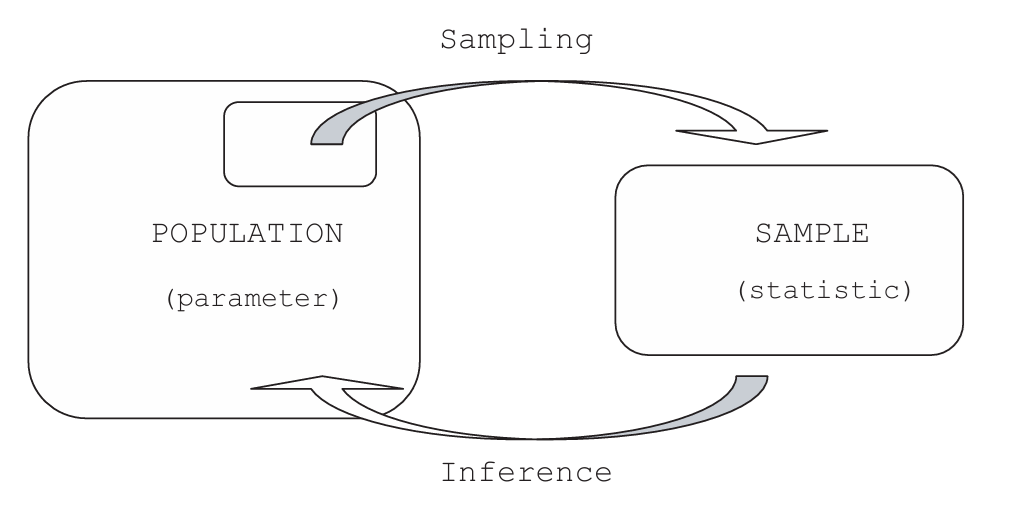
\includegraphics[keepaspectratio]{figs/ch1/inference.png}}

}

\caption{\label{fig-inference}Statistical Inference}

\end{figure}%

In practice, what a statistician is often interested in is a
\textbf{population}---a collection of all possible individuals, objects,
or measurements of interest. Of particular importance is some numerical
characteristic of the population, known as a \textbf{parameter}.

Because it is usually impossible (or impractical) to observe the entire
population, a \textbf{sample} is drawn. From this sample, a
\textbf{statistic}---a numerical quantity describing some feature of the
sample---is calculated. Statistical inference then uses this statistic
to say something about the corresponding population parameter.

Before we treat inferential statistics later in this book in detail, we
begin with a discussion of basic statistical concepts that are best
introduced through descriptive statistics, together with an introduction
to elementary probability, which is essential for understanding
statistical inference.

\section{Pioneers of statistics}\label{pioneers-of-statistics}

There are several approaches to doing statistics. In this book, we
primarily adopt the \textbf{classical approach}, developed largely by
\textbf{Sir Ronald Aylmer Fisher (1890--1962)}---a British statistician,
geneticist, and professor. For his contributions, Fisher has been
described as \emph{``a genius who almost single-handedly created the
foundations for modern statistical science.''} (Efron 1998)

Another important framework is the \textbf{Bayesian approach},
associated with \textbf{Thomas Bayes (1702--1761)}, an English
statistician, philosopher, and Presbyterian minister. Bayes is best
known for formulating what is now called \textbf{Bayes' theorem}, which
will be introduced in a later chapter.\footnote{Interestingly, Bayes
  never published what would become his most famous accomplishment; his
  notes were edited and published after his death by Richard Price.}

\begin{center}\rule{0.5\linewidth}{0.5pt}\end{center}

\section{Key terms}\label{key-terms}

\subsection{Data}\label{data}

Data are characteristics or pieces of information---usually
numerical---collected through observation. More formally, \textbf{data}
are sets of values of qualitative or quantitative variables measured on
one or more individuals or objects. A \textbf{datum} (the singular of
data) refers to a single value of a single variable.

\subsection{Statistics}\label{statistics}

Statistics is the discipline concerned with the \textbf{collection,
organization, analysis, interpretation, and presentation of data}.

\subsection{Descriptive statistics}\label{descriptive-statistics}

Descriptive statistics refers to the process of \textbf{summarizing and
describing data}, typically using tables, graphs, and numerical
measures.

\subsection{Inferential statistics}\label{inferential-statistics}

Inferential statistics (or statistical inference) is the process of
\textbf{using data from a sample to draw conclusions about an underlying
population or probability distribution}.

\begin{tcolorbox}[enhanced jigsaw, coltitle=black, colbacktitle=quarto-callout-important-color!10!white, left=2mm, bottomrule=.15mm, bottomtitle=1mm, colback=white, titlerule=0mm, colframe=quarto-callout-important-color-frame, breakable, leftrule=.75mm, toptitle=1mm, opacitybacktitle=0.6, rightrule=.15mm, title=\textcolor{quarto-callout-important-color}{\faExclamation}\hspace{0.5em}{Chapter summary}, arc=.35mm, opacityback=0, toprule=.15mm]

Statistics provides tools for turning raw data into meaningful
information.

Descriptive statistics summarize and present data, while inferential
statistics use data from samples to draw conclusions about populations.
Central to statistical reasoning are the ideas of populations, samples,
parameters, and statistics, as well as the role of probability in making
inference possible.

This chapter sets the conceptual foundation for the rest of the book and
motivates the need for the descriptive and inferential tools developed
in later chapters.

\end{tcolorbox}

\bookmarksetup{startatroot}

\chapter{Graphical Summaries}\label{ch2}

\begin{tcolorbox}[enhanced jigsaw, coltitle=black, colbacktitle=quarto-callout-note-color!10!white, left=2mm, bottomrule=.15mm, bottomtitle=1mm, colback=white, titlerule=0mm, colframe=quarto-callout-note-color-frame, breakable, leftrule=.75mm, toptitle=1mm, opacitybacktitle=0.6, rightrule=.15mm, title=\textcolor{quarto-callout-note-color}{\faInfo}\hspace{0.5em}{Learning objectives}, arc=.35mm, opacityback=0, toprule=.15mm]

By the end of this chapter, you should be able to:

\begin{itemize}
\tightlist
\item
  explain why graphical summaries are useful for understanding data,
\item
  distinguish between cardinal, ordinal, and nominal data,
\item
  identify appropriate graphical representations for different types of
  data,
\item
  construct and interpret histograms correctly, including those with
  unequal class intervals,
\item
  explain how histogram areas represent percentages or probabilities,
\item
  recognize common histogram shapes such as symmetric, skewed, unimodal,
  and bimodal distributions.
\end{itemize}

\end{tcolorbox}

A defining characteristic of today's information age is the abundance of
data. Data in their raw form can be difficult to comprehend. One useful
way to summarize a mass of data is through \textbf{graphical or
pictorial representations}.

Many such graphs---pie charts, bar graphs, and so on---are easy to
understand and commonly used. In this chapter, we focus on the
\textbf{most important graphical representation in statistics: the
histogram}.\footnote{Why might graphs be more informative than tables
  when data sets are large?}\{.sidenote\}

\begin{tcolorbox}[enhanced jigsaw, coltitle=black, colbacktitle=quarto-callout-note-color!10!white, left=2mm, bottomrule=.15mm, bottomtitle=1mm, colback=white, titlerule=0mm, colframe=quarto-callout-note-color-frame, breakable, leftrule=.75mm, toptitle=1mm, opacitybacktitle=0.6, rightrule=.15mm, title=\textcolor{quarto-callout-note-color}{\faInfo}\hspace{0.5em}{Big picture}, arc=.35mm, opacityback=0, toprule=.15mm]

Graphs help us \emph{see} patterns in data that are often invisible in
raw numbers.

\end{tcolorbox}

\section{Types of data}\label{types-of-data}

Data are not all the same. A helpful way to think about them is in
\textbf{three levels}:

\begin{itemize}
\tightlist
\item
  \textbf{Cardinal data}
\item
  \textbf{Ordinal data}
\item
  \textbf{Nominal data}
\end{itemize}

Once you know which kind of data you have, it becomes much easier to
choose sensible statistics and graphs.

\subsection{Cardinal data}\label{cardinal-data}

\textbf{Cardinal data} (sometimes further divided into \emph{interval}
and \emph{ratio} data) are represented by real numbers---such as
heights, weights, and prices. These are \textbf{quantitative
(numerical)} data, so arithmetic operations are meaningful.

For example, with heights or prices, it makes sense to say someone is
\emph{twice as tall} or that one item is \emph{three times as
expensive}.

\subsection{Ordinal data}\label{ordinal-data}

\textbf{Ordinal data} are values for which \textbf{only the order
(ranking)} is meaningful. A common example is a course evaluation scale
such as:

\begin{itemize}
\tightlist
\item
  Poor = 1\\
\item
  Fair = 2\\
\item
  Good = 3\\
\item
  Very Good = 4\\
\item
  Excellent = 5
\end{itemize}

Here, arithmetic operations usually do \textbf{not} make sense. It would
sound strange, for instance, to say:

\texttt{2\ ×\ Fair\ =\ Very\ Good}.

Still, ordinal data are useful because the ranking is clear:
\emph{Excellent} (5) is better than \emph{Very Good} (4), which is
better than \emph{Good} (3), and so on. Importantly, that ordering
remains the same even if we changed the numbers used to label the
categories.

\subsection{Nominal data}\label{nominal-data}

\textbf{Nominal data} are usually \textbf{qualitative or categorical}.
The numbers attached to categories serve only as labels. For example,
marital status might be coded as:

\begin{itemize}
\tightlist
\item
  Single = 1\\
\item
  Married = 2\\
\item
  Divorced = 3\\
\item
  Widowed = 4
\end{itemize}

Because these numbers are arbitrary, arithmetic operations are
meaningless. It is absurd, for example, to say:

\texttt{married\ ÷\ 2\ =\ single}.

With categorical data, the main meaningful calculation is
\textbf{counting}---how often each category occurs. We often summarize
nominal data using a \textbf{frequency distribution}, or a
\textbf{relative frequency distribution} showing proportions.

\begin{tcolorbox}[enhanced jigsaw, coltitle=black, colbacktitle=quarto-callout-important-color!10!white, left=2mm, bottomrule=.15mm, bottomtitle=1mm, colback=white, titlerule=0mm, colframe=quarto-callout-important-color-frame, breakable, leftrule=.75mm, toptitle=1mm, opacitybacktitle=0.6, rightrule=.15mm, title=\textcolor{quarto-callout-important-color}{\faExclamation}\hspace{0.5em}{Key idea}, arc=.35mm, opacityback=0, toprule=.15mm]

The \emph{type} of data determines which graphs and summaries make
sense.

\end{tcolorbox}

\subsection{Why this matters}\label{why-this-matters}

Keeping the data type in mind helps determine which statistical
tools---graphical or otherwise---are appropriate. Among graphical
techniques, we will emphasize the \textbf{histogram}, which plays a
central role in statistics and probability.

\section{The histogram}\label{the-histogram}

To understand how a histogram works, let us look at a concrete
example.\\
Table~\ref{tbl-income} shows the \textbf{percentage of families} in each
\textbf{income class interval}, measured in thousands of baht per year,
for Bangkok residents in a recent year.

\begin{longtable}[]{@{}ll@{}}
\caption{Annual income for a sample of Bangkok
residents}\label{tbl-income}\tabularnewline
\toprule\noalign{}
Income (Baht '000) & Percentage \\
\midrule\noalign{}
\endfirsthead
\toprule\noalign{}
Income (Baht '000) & Percentage \\
\midrule\noalign{}
\endhead
\bottomrule\noalign{}
\endlastfoot
0--30 & 1 \\
30--60 & 3 \\
60--90 & 6 \\
90--120 & 10 \\
120--150 & 11 \\
150--210 & 24 \\
210--270 & 20 \\
270--390 & 18 \\
390--600 & 5 \\
Over 600 & 1 \\
\end{longtable}

To construct a histogram from Table~\ref{tbl-income}, the \textbf{first
step} is to draw the \textbf{horizontal axis}, representing income.

A common mistake at this stage is to give \textbf{each class interval
the same width}, regardless of its actual size. This leads to a
misleading picture.

\pandocbounded{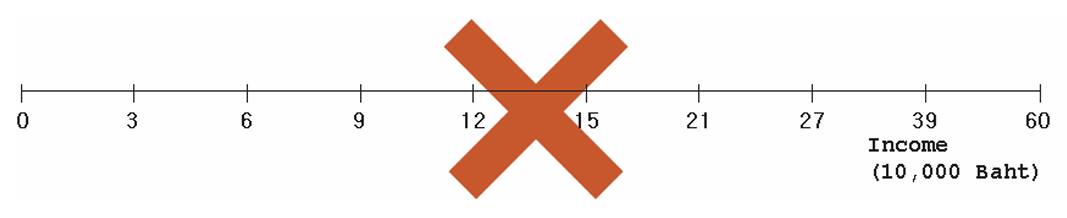
\includegraphics[keepaspectratio]{figs/ch2/vert-a.png}}

Instead, the horizontal axis should reflect the \emph{actual width} of
each income class, as shown below.\footnote{Class intervals need not be
  equal; wider intervals may be used where data are sparse.}

\pandocbounded{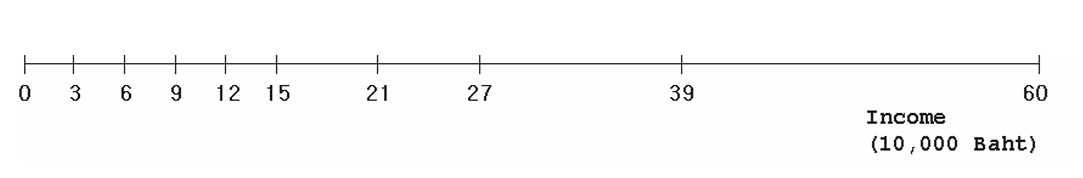
\includegraphics[keepaspectratio]{figs/ch2/vert-b.png}}

The next step is to draw the blocks. Students often make the mistake of
setting the height of each block equal to the percentage in the table.
The figure below shows what happens if this is done.

\pandocbounded{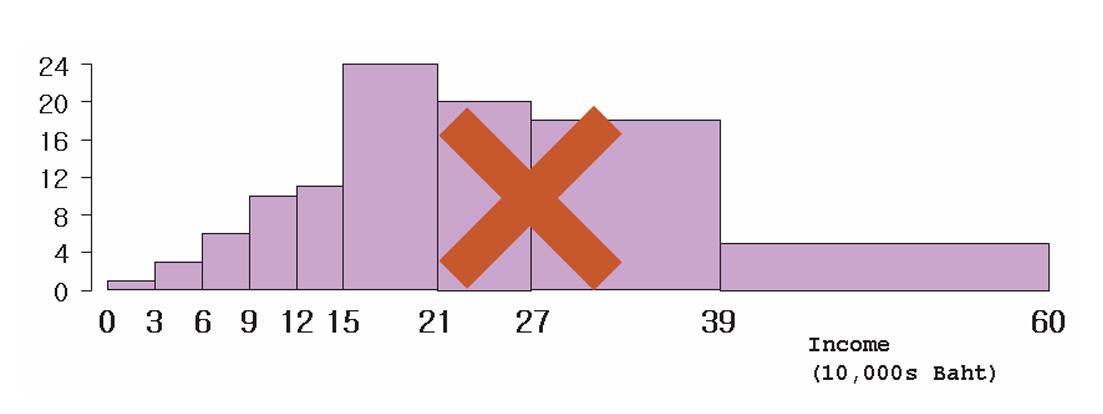
\includegraphics[keepaspectratio]{figs/ch2/hist-a.png}}

This gives a misleading impression---for example, it appears that there
are more families earning over 390,000 baht than under 120,000 baht,
which is not correct.

\begin{tcolorbox}[enhanced jigsaw, coltitle=black, colbacktitle=quarto-callout-warning-color!10!white, left=2mm, bottomrule=.15mm, bottomtitle=1mm, colback=white, titlerule=0mm, colframe=quarto-callout-warning-color-frame, breakable, leftrule=.75mm, toptitle=1mm, opacitybacktitle=0.6, rightrule=.15mm, title=\textcolor{quarto-callout-warning-color}{\faExclamationTriangle}\hspace{0.5em}{Common pitfall}, arc=.35mm, opacityback=0, toprule=.15mm]

In a histogram, \textbf{heights alone do not represent frequencies} when
class widths differ.

\end{tcolorbox}

Because the class intervals are unequal, the height of each block must
be calculated as:

\begin{quote}
percentage ÷ class width (relative length)
\end{quote}

For example, the interval 150--210 spans two 30,000-baht units. Dividing
24\% by 2 gives the correct height. The vertical axis is therefore a
\textbf{density scale} (percent per 30,000). The correct histogram is:

\begin{figure}

\centering{

\pandocbounded{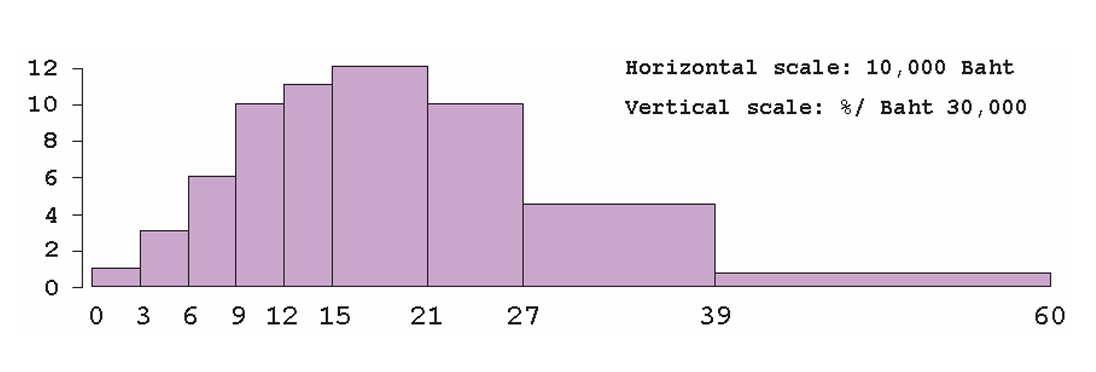
\includegraphics[keepaspectratio]{figs/ch2/hist-b.png}}

}

\caption{\label{fig-correcthist}Correct Histogram}

\end{figure}%

In a histogram: - \textbf{areas} represent percentages (or
probabilities) - \textbf{heights} represent crowding per horizontal unit

An important property to remember is that the \textbf{total area under
the histogram must equal 100 percent}.

\begin{tcolorbox}[enhanced jigsaw, coltitle=black, colbacktitle=quarto-callout-important-color!10!white, left=2mm, bottomrule=.15mm, bottomtitle=1mm, colback=white, titlerule=0mm, colframe=quarto-callout-important-color-frame, breakable, leftrule=.75mm, toptitle=1mm, opacitybacktitle=0.6, rightrule=.15mm, title=\textcolor{quarto-callout-important-color}{\faExclamation}\hspace{0.5em}{Key idea}, arc=.35mm, opacityback=0, toprule=.15mm]

Histograms represent data through \emph{areas}, not just heights.

\end{tcolorbox}

\section{Shapes of histograms}\label{shapes-of-histograms}

Histograms come in many shapes. A histogram is \textbf{symmetric} if the
two sides mirror each other around a central vertical line. The most
famous symmetric histogram is the \textbf{Gaussian (normal)
distribution}.

\begin{figure}

\centering{

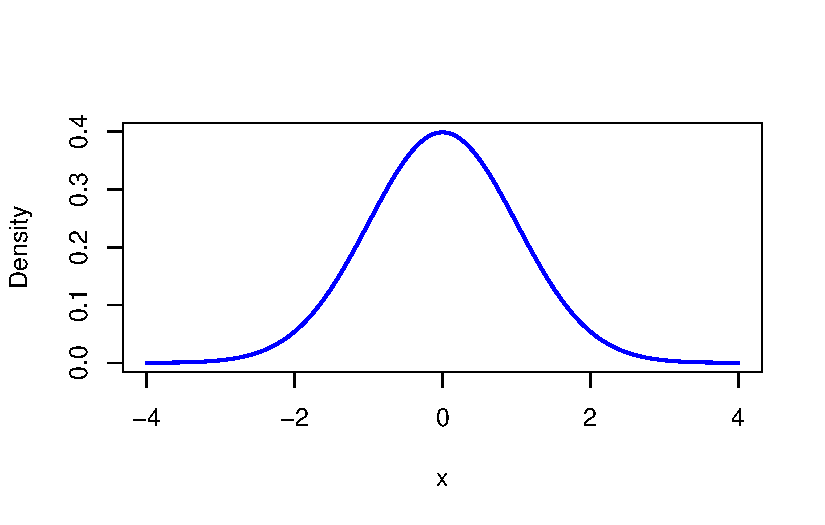
\includegraphics[width=0.75\linewidth,height=\textheight,keepaspectratio]{Ch2_files/figure-pdf/fig-gaussian-1.pdf}

}

\caption{\label{fig-gaussian}Gaussian Distribution}

\end{figure}%

A \textbf{skewed histogram} is one with a long tail extending either to
the right or to the left:

\begin{center}
\pandocbounded{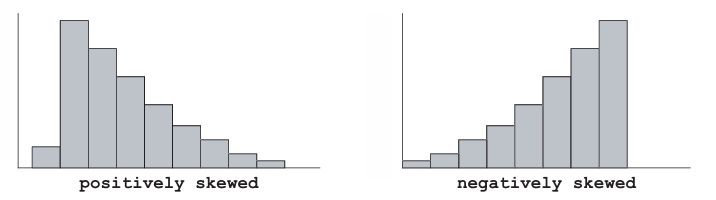
\includegraphics[keepaspectratio]{figs/ch2/skewed.png}}
\end{center}

Histograms can also be \textbf{unimodal}, with a single peak, or
\textbf{bimodal}, with two peaks, and so on.

\begin{center}
\pandocbounded{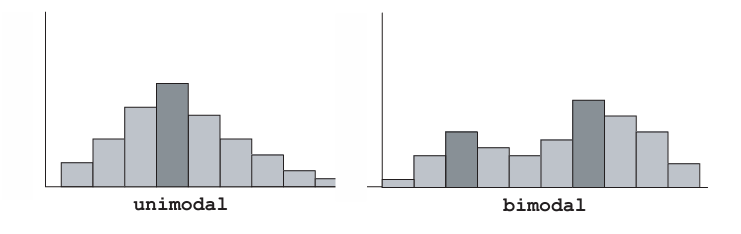
\includegraphics[keepaspectratio]{figs/ch2/modal.png}}
\end{center}

\begin{tcolorbox}[enhanced jigsaw, coltitle=black, colbacktitle=quarto-callout-important-color!10!white, left=2mm, bottomrule=.15mm, bottomtitle=1mm, colback=white, titlerule=0mm, colframe=quarto-callout-important-color-frame, breakable, leftrule=.75mm, toptitle=1mm, opacitybacktitle=0.6, rightrule=.15mm, title=\textcolor{quarto-callout-important-color}{\faExclamation}\hspace{0.5em}{Key idea}, arc=.35mm, opacityback=0, toprule=.15mm]

The \emph{shape} of a histogram provides valuable information about the
distribution of the data, beyond what summary statistics alone can
reveal.

\end{tcolorbox}

\section{Quantitative and qualitative
variables}\label{quantitative-and-qualitative-variables}

A \textbf{variable} is a characteristic that can vary from one
individual to another.\\
For example, if we ask \emph{``How old are you?''}, the variable of
interest is \textbf{age}.\\
In this case, age is a \emph{quantitative variable}, since it is usually
expressed as a number.

In other cases, the question might be \emph{``What color is your
hair?''}\\
Here, the variable is a \emph{qualitative variable}, because the
responses describe categories rather than numerical magnitudes.

A useful distinction among quantitative variables is between
\textbf{discrete} and \textbf{continuous} variables.

\begin{itemize}
\tightlist
\item
  A \textbf{discrete variable} takes on values in fixed steps. An
  example is the number of children in a household.
\item
  A \textbf{continuous variable} can take on any value along a real
  line, such as height, weight, or income.
\end{itemize}

Working with quantitative variables is usually straightforward.
Qualitative variables, however, are often handled by assigning
\textbf{arbitrary numerical codes} to the possible responses. In
practice, this means that a researcher codes qualitative information
into nominal numerical data.

For example, a course evaluation might be coded as:

\begin{itemize}
\tightlist
\item
  Poor = 1\\
\item
  Fair = 2\\
\item
  Good = 3\\
\item
  Very Good = 4\\
\item
  Excellent = 5
\end{itemize}

\begin{tcolorbox}[enhanced jigsaw, coltitle=black, colbacktitle=quarto-callout-warning-color!10!white, left=2mm, bottomrule=.15mm, bottomtitle=1mm, colback=white, titlerule=0mm, colframe=quarto-callout-warning-color-frame, breakable, leftrule=.75mm, toptitle=1mm, opacitybacktitle=0.6, rightrule=.15mm, title=\textcolor{quarto-callout-warning-color}{\faExclamationTriangle}\hspace{0.5em}{Common pitfall}, arc=.35mm, opacityback=0, toprule=.15mm]

Do not treat coded qualitative variables as numerical measurements.
Arithmetic operations on these codes usually have no meaningful
interpretation.

\end{tcolorbox}

It is important to remember that these numbers are \textbf{labels rather
than true measurements}, and arithmetic operations on them may not be
meaningful.

It is also useful to distinguish between different \textbf{data
structures}, such as:

\begin{itemize}
\tightlist
\item
  \textbf{Cross-sectional data}, which observe many individuals at a
  single point in time\\
\item
  \textbf{Time-series data}, which track a single unit over time\\
\item
  \textbf{Panel (or longitudinal) data}, which follow multiple
  individuals over time
\end{itemize}

The statistical tools available to the researcher often depend on which
of these data structures is being used.

\begin{tcolorbox}[enhanced jigsaw, coltitle=black, colbacktitle=quarto-callout-note-color!10!white, left=2mm, bottomrule=.15mm, bottomtitle=1mm, colback=white, titlerule=0mm, colframe=quarto-callout-note-color-frame, breakable, leftrule=.75mm, toptitle=1mm, opacitybacktitle=0.6, rightrule=.15mm, title=\textcolor{quarto-callout-note-color}{\faInfo}\hspace{0.5em}{Pause and think}, arc=.35mm, opacityback=0, toprule=.15mm]

Which of the variables you encounter in daily life---income, grades, or
job titles---are quantitative, and which are qualitative?

\end{tcolorbox}

\section{Other graphical representations of
data}\label{other-graphical-representations-of-data}

There are many graphical methods available for representing data. Some,
such as \textbf{bar graphs} and \textbf{pie charts}, are widely known.
Others, such as the \textbf{stem-and-leaf plot} or the \textbf{ogive},
are more specialized.

Most introductory statistics textbooks discuss a variety of graphical
summaries, and interested readers are encouraged to consult these
sources.\footnote{Some recommended texts include Peck, Olsen, and Devore
  (2005, Chapter 3), Utts and Heckard (2006, Chapter 2), and Keller
  (2005, Chapters 2 and 3). The exercises at the end of this book also
  ask for graphical summaries not fully explained here, but which are
  worth exploring with the help of other introductory texts or online
  resources.}

\begin{tcolorbox}[enhanced jigsaw, coltitle=black, colbacktitle=quarto-callout-important-color!10!white, left=2mm, bottomrule=.15mm, bottomtitle=1mm, colback=white, titlerule=0mm, colframe=quarto-callout-important-color-frame, breakable, leftrule=.75mm, toptitle=1mm, opacitybacktitle=0.6, rightrule=.15mm, title=\textcolor{quarto-callout-important-color}{\faExclamation}\hspace{0.5em}{Big picture}, arc=.35mm, opacityback=0, toprule=.15mm]

Many graphical tools exist, but for understanding distributions and
probabilities, the \textbf{histogram} plays a uniquely central role.

\end{tcolorbox}

\begin{tcolorbox}[enhanced jigsaw, coltitle=black, colbacktitle=quarto-callout-important-color!10!white, left=2mm, bottomrule=.15mm, bottomtitle=1mm, colback=white, titlerule=0mm, colframe=quarto-callout-important-color-frame, breakable, leftrule=.75mm, toptitle=1mm, opacitybacktitle=0.6, rightrule=.15mm, title=\textcolor{quarto-callout-important-color}{\faExclamation}\hspace{0.5em}{Chapter summary}, arc=.35mm, opacityback=0, toprule=.15mm]

Graphical summaries provide a powerful way to explore and communicate
patterns in data.

Different types of data---cardinal, ordinal, and nominal---call for
different graphical representations. Among these, the histogram plays a
central role in statistics because it summarizes distributions through
areas and connects naturally to ideas of probability.

Understanding how to construct and interpret histograms, especially when
class intervals are unequal, is essential for sound statistical analysis
and for the topics that follow in later chapters.

\end{tcolorbox}

\begin{center}\rule{0.5\linewidth}{0.5pt}\end{center}

\section{Exercises}\label{exercises}

\subsection{Conceptual questions}\label{conceptual-questions}

\begin{enumerate}
\def\labelenumi{\arabic{enumi}.}
\item
  Explain why graphical summaries are often more informative than tables
  when dealing with large data sets.
\item
  Give one example each of:

  \begin{itemize}
  \tightlist
  \item
    a cardinal variable,
  \item
    an ordinal variable, and
  \item
    a nominal variable.
  \end{itemize}

  Briefly explain why arithmetic operations make sense for one but not
  for the others.
\item
  Why can assigning numbers to qualitative categories be misleading if
  those numbers are treated as measurements?
\item
  A histogram shows two distributions with the same total area. What
  does this tell you about the data being represented?
\end{enumerate}

\begin{tcolorbox}[enhanced jigsaw, coltitle=black, colbacktitle=quarto-callout-note-color!10!white, left=2mm, bottomrule=.15mm, bottomtitle=1mm, colback=white, titlerule=0mm, colframe=quarto-callout-note-color-frame, breakable, leftrule=.75mm, toptitle=1mm, opacitybacktitle=0.6, rightrule=.15mm, title=\textcolor{quarto-callout-note-color}{\faInfo}\hspace{0.5em}{Check your understanding}, arc=.35mm, opacityback=0, toprule=.15mm]

If two histograms look very different but have the same total area, what
does this imply about the percentages or probabilities they represent?

\end{tcolorbox}

\begin{center}\rule{0.5\linewidth}{0.5pt}\end{center}

\subsection{Interpreting histograms}\label{interpreting-histograms}

\begin{enumerate}
\def\labelenumi{\arabic{enumi}.}
\setcounter{enumi}{4}
\tightlist
\item
  Consider a histogram constructed using unequal class intervals.

  \begin{itemize}
  \tightlist
  \item
    Why must the vertical axis be interpreted as a \emph{density} rather
    than a raw frequency?
  \item
    What would go wrong if heights were drawn directly from percentages?
  \end{itemize}
\item
  A histogram is right-skewed.

  \begin{itemize}
  \tightlist
  \item
    What does this tell you about the distribution of the data?
  \item
    Give a real-world example of a variable that is likely to be
    right-skewed.
  \end{itemize}
\item
  Explain the difference between a unimodal and a bimodal histogram.\\
  What might cause a bimodal shape in real data?
\item
  The histogram below shows the distribution of final scores in a
  certain class.\\
  \begin{center}
  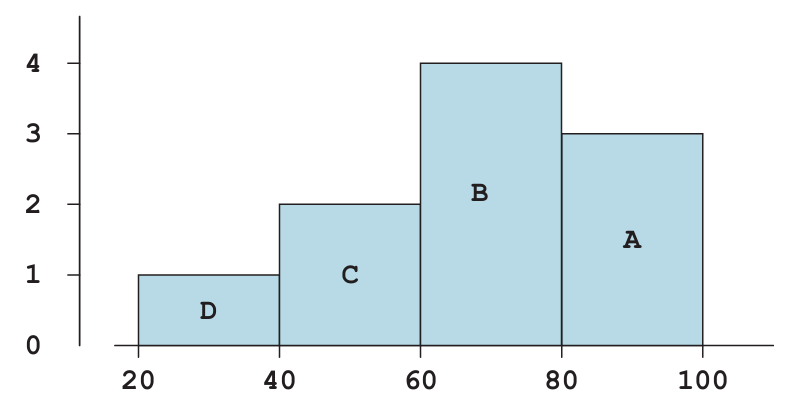
\includegraphics[width=0.5\linewidth,height=\textheight,keepaspectratio]{figs/exercise/ws-2-8.png}
  \end{center}

  \begin{itemize}
  \tightlist
  \item
    which block represents the people who scored between 60 and 80?
  \item
    Ten percent scored between 20 and 40. About what percentage scored
    between 40 and 60?
  \item
    About what percentage scored over 60?\\
    9.A histogram of pocket-money used by EBA students in a week is
    shown above. No student used over Baht1,000 per month. The block
    over the class interval 200-500 is missing. How tall must it be?\\
    \pandocbounded{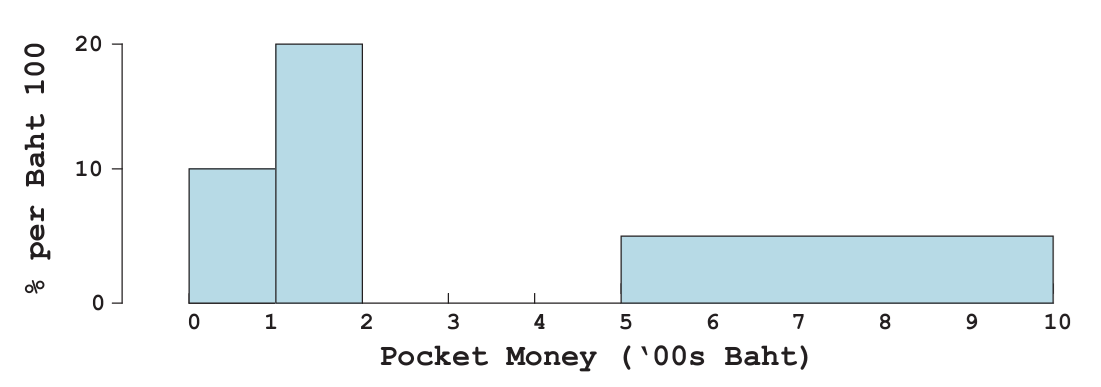
\includegraphics[keepaspectratio]{figs/exercise/ws-2-9.png}}
  \end{itemize}
\item
  The figure below shows a block of family income in a certain town.
  About what percent of the families in the city had incomes between
  Baht 15,000 and 25,000?\\
  \begin{center}
  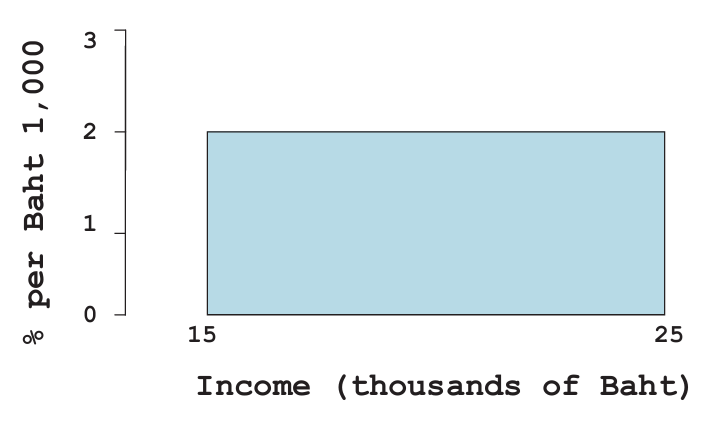
\includegraphics[width=0.5\linewidth,height=\textheight,keepaspectratio]{figs/exercise/ws-2-10.png}
  \end{center}
\end{enumerate}

\begin{tcolorbox}[enhanced jigsaw, coltitle=black, colbacktitle=quarto-callout-warning-color!10!white, left=2mm, bottomrule=.15mm, bottomtitle=1mm, colback=white, titlerule=0mm, colframe=quarto-callout-warning-color-frame, breakable, leftrule=.75mm, toptitle=1mm, opacitybacktitle=0.6, rightrule=.15mm, title=\textcolor{quarto-callout-warning-color}{\faExclamationTriangle}\hspace{0.5em}{Common pitfall}, arc=.35mm, opacityback=0, toprule=.15mm]

Students often confuse the \emph{height} of bars with the \emph{area} of
bars in a histogram.

\end{tcolorbox}

\begin{center}\rule{0.5\linewidth}{0.5pt}\end{center}

\subsection{Data structure and graphs}\label{data-structure-and-graphs}

\begin{enumerate}
\def\labelenumi{\arabic{enumi}.}
\setcounter{enumi}{10}
\tightlist
\item
  For each of the following data structures, suggest an appropriate
  graphical summary and explain why: - cross-sectional data, -
  time-series data, - panel (longitudinal) data.
\item
  Why is the histogram particularly important for later topics in
  probability and statistical inference?
\end{enumerate}

\begin{center}\rule{0.5\linewidth}{0.5pt}\end{center}

\subsection{Optional challenge}\label{optional-challenge}

\begin{enumerate}
\def\labelenumi{\arabic{enumi}.}
\setcounter{enumi}{12}
\tightlist
\item
  Find a real dataset (from news, government statistics, or online
  sources) and:

  \begin{itemize}
  \tightlist
  \item
    classify the variables as cardinal, ordinal, or nominal,
  \item
    propose at least one appropriate graphical summary for each
    variable,
  \item
    explain why a histogram would or would not be appropriate.
  \end{itemize}
\end{enumerate}

\bookmarksetup{startatroot}

\chapter{Numerical Summaries}\label{ch3}

\begin{tcolorbox}[enhanced jigsaw, coltitle=black, colbacktitle=quarto-callout-note-color!10!white, left=2mm, bottomrule=.15mm, bottomtitle=1mm, colback=white, titlerule=0mm, colframe=quarto-callout-note-color-frame, breakable, leftrule=.75mm, toptitle=1mm, opacitybacktitle=0.6, rightrule=.15mm, title=\textcolor{quarto-callout-note-color}{\faInfo}\hspace{0.5em}{Learning objectives}, arc=.35mm, opacityback=0, toprule=.15mm]

By the end of this chapter, you should be able to:

\begin{itemize}
\tightlist
\item
  explain the purpose of numerical summaries in descriptive statistics,
\item
  distinguish between different measures of central location,
\item
  describe how dispersion captures variability in data,
\item
  compute and interpret the mean, median, and standard deviation,
\item
  explain the difference between population and sample standard
  deviation,
\item
  interpret percentiles and quartiles as measures of relative standing.
\end{itemize}

\end{tcolorbox}

Descriptive statistics consist not only of graphical summaries, but also
of \textbf{numerical methods}.\\
Since we introduced the histogram in the previous chapter---the most
important graphical summary of data---we now turn to \textbf{basic
numerical descriptive statistics}.

These include:

\begin{itemize}
\tightlist
\item
  \textbf{Measures of central location}, such as the mean, median, and
  mode\\
\item
  \textbf{Measures of dispersion (or spread)}, such as the range,
  variance, standard deviation, and coefficient of variation\\
\item
  \textbf{Measures of relative standing}, such as percentiles and
  quartiles
\end{itemize}

Together, these numerical summaries help us describe data in a concise
and informative way.

\begin{tcolorbox}[enhanced jigsaw, coltitle=black, colbacktitle=quarto-callout-note-color!10!white, left=2mm, bottomrule=.15mm, bottomtitle=1mm, colback=white, titlerule=0mm, colframe=quarto-callout-note-color-frame, breakable, leftrule=.75mm, toptitle=1mm, opacitybacktitle=0.6, rightrule=.15mm, title=\textcolor{quarto-callout-note-color}{\faInfo}\hspace{0.5em}{Big picture}, arc=.35mm, opacityback=0, toprule=.15mm]

Numerical summaries allow us to describe large datasets using just a few
carefully chosen numbers.

\end{tcolorbox}

\section{Measure of central location}\label{measure-of-central-location}

The \textbf{arithmetic mean} (or simply, the \emph{average}) is the most
widely used measure of central location. It is calculated by adding up
all observed values and dividing by the number of observations.

\begin{equation}\phantomsection\label{eq-mean}{
\overline{X} = \frac{1}{n} \sum_{i=1}^{n} X_i
}\end{equation}

The arithmetic mean, shown formally as Equation~\ref{eq-mean}, is
\textbf{unique}. Moreover, it has an important and intuitive property:
the sum of the deviations of each observation from the mean is zero.

An interesting way to visualize this property is through a histogram. If
the histogram were placed on a balance, it would balance exactly when
supported at the arithmetic mean.

\pandocbounded{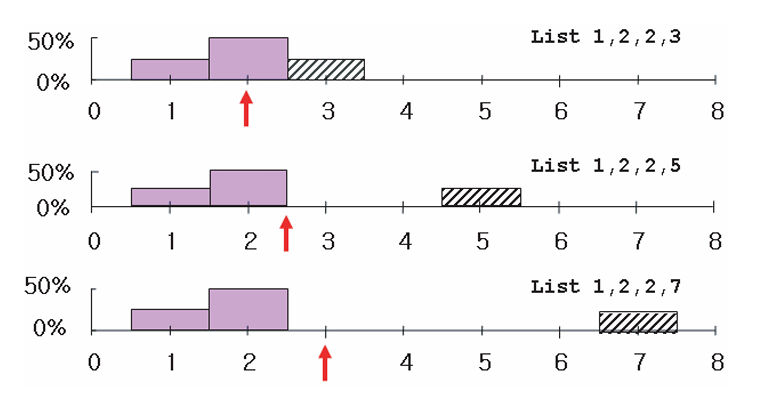
\includegraphics[keepaspectratio]{figs/ch3/mean.png}}

The \textbf{median}, another measure of central location, is the
midpoint of the values in a dataset once the observations are ordered
from the smallest to the largest.

The \textbf{mode} is a less commonly used measure of central location
and refers to the value that occurs most frequently in the data.

An important advantage of the median is that it is \textbf{not affected
by extremely large or small values}. For this reason, it is often a more
reliable measure of central location when such extreme values are
present.

The mode, on the other hand, can be interpreted as the \emph{``fashion
category''} of the data. In a histogram, it corresponds to the tallest
bar or the highest peak.

\begin{tcolorbox}[enhanced jigsaw, coltitle=black, colbacktitle=quarto-callout-important-color!10!white, left=2mm, bottomrule=.15mm, bottomtitle=1mm, colback=white, titlerule=0mm, colframe=quarto-callout-important-color-frame, breakable, leftrule=.75mm, toptitle=1mm, opacitybacktitle=0.6, rightrule=.15mm, title=\textcolor{quarto-callout-important-color}{\faExclamation}\hspace{0.5em}{Key idea}, arc=.35mm, opacityback=0, toprule=.15mm]

The mean, median, and mode summarize the \emph{center} of the data, but
they respond differently to extreme values.

\end{tcolorbox}

For \textbf{symmetrical histograms}, such as the Gaussian (normal)
distribution, the three measures coincide:

\[
\text{mean} = \text{median} = \text{mode}.
\]

\begin{center}
\pandocbounded{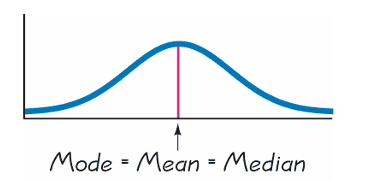
\includegraphics[keepaspectratio]{figs/ch3/no-skew.png}}
\end{center}

But not all histograms are symmetric. If a histogram is skewed to the
left or to the right, the three measures may differ.

\pandocbounded{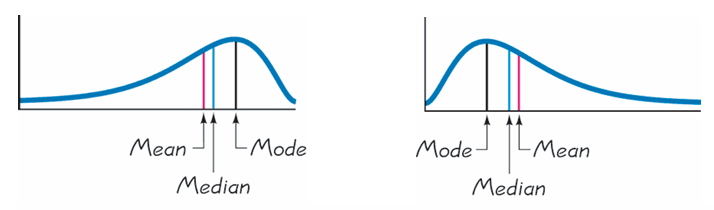
\includegraphics[keepaspectratio]{figs/ch3/skew.png}}

What is important to realize is that \textbf{extreme values affect the
average most, then the median, and least the mode}. The arithmetic mean
is therefore the most sensitive to extremely large or small values.

\begin{tcolorbox}[enhanced jigsaw, coltitle=black, colbacktitle=quarto-callout-warning-color!10!white, left=2mm, bottomrule=.15mm, bottomtitle=1mm, colback=white, titlerule=0mm, colframe=quarto-callout-warning-color-frame, breakable, leftrule=.75mm, toptitle=1mm, opacitybacktitle=0.6, rightrule=.15mm, title=\textcolor{quarto-callout-warning-color}{\faExclamationTriangle}\hspace{0.5em}{Common pitfall}, arc=.35mm, opacityback=0, toprule=.15mm]

Relying only on the mean can be misleading when the data contain extreme
values or are highly skewed.

\end{tcolorbox}

\section{Measures of dispersion or
spread}\label{measures-of-dispersion-or-spread}

\pandocbounded{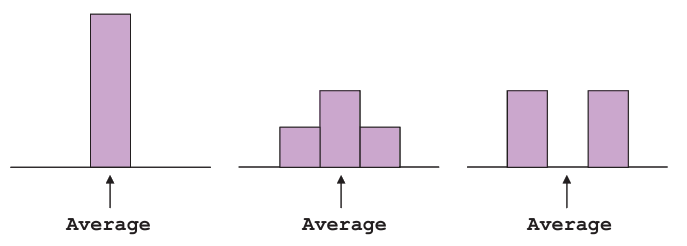
\includegraphics[keepaspectratio]{figs/ch3/mean-not-enough.png}}

The three histograms above all have the same average (or mean), yet they
clearly look different. Describing a distribution using only its mean is
therefore not sufficient. We also need to know how \textbf{spread out}
the data are---that is, the \textbf{dispersion} or \textbf{variability}
of the observations.

There are many measures of dispersion, including the range, the mean
absolute deviation, the root mean square (r.m.s.), the standard
deviation, the variance, the coefficient of variation, and the
interquartile range. We now focus on the most important of these.

\subsection{The standard deviation}\label{the-standard-deviation}

The \textbf{standard deviation}, abbreviated as \textbf{SD}, is the most
important measure of dispersion used in this book. There are several
ways to define and compute it, but the most intuitive approach is based
on the idea of the \textbf{root mean square (r.m.s.)}.

The starting point is the notion of a \textbf{deviation}, which is
simply the distance of an observation from the average. Mathematically,
the deviation of an observation (\(X_i\)) from the mean
(\(\overline{X}\)) is

\[
\text{deviation} = X_i - \overline{X}.
\]

The term \textbf{root mean square} is a useful reminder of the steps
involved---provided one reads it backwards:

\begin{enumerate}
\def\labelenumi{\arabic{enumi}.}
\tightlist
\item
  \textbf{Square} all the entries\\
\item
  Take the \textbf{mean} of the squares\\
\item
  Take the square \textbf{root} of the mean
\end{enumerate}

In equation form, the root mean square of a variable \(X\) can be
written as

\[
\text{r.m.s. of } X = \sqrt{X^2}.
\]

This, however, is just a \emph{mathematical operation}.

The \textbf{standard deviation} is defined more specifically as the root
mean square of the \textbf{deviations from the mean}, that is,

\[
\text{SD of } X = \text{r.m.s. (deviation from the average)}.
\]

In simple terms, the standard deviation tells us how far, on average,
the observations lie from their mean.

\subsection{A numerical example}\label{a-numerical-example}

To make this concrete, consider the list of numbers

\[
20,\; 10,\; 15,\; 15.
\]

The average \(\overline{X}\) is 15. The deviations from the mean are
therefore

\[
5,\; -5,\; 0,\; 0.
\]

Applying the r.m.s. procedure gives the standard deviation:

\[
\begin{aligned}
\text{SD}
&= \sqrt{\frac{5^2 + (-5)^2 + 0^2 + 0^2}{4}} \\
&= \sqrt{\frac{25 + 25 + 0 + 0}{4}} \\
&= \sqrt{\frac{50}{4}} = \sqrt{12.5} \approx 3.5.
\end{aligned}
\]

\begin{tcolorbox}[enhanced jigsaw, coltitle=black, colbacktitle=quarto-callout-tip-color!10!white, left=2mm, bottomrule=.15mm, bottomtitle=1mm, colback=white, titlerule=0mm, colframe=quarto-callout-tip-color-frame, breakable, leftrule=.75mm, toptitle=1mm, opacitybacktitle=0.6, rightrule=.15mm, title=\textcolor{quarto-callout-tip-color}{\faLightbulb}\hspace{0.5em}{Try This: Exploring Mean and SD}, arc=.35mm, opacityback=0, toprule=.15mm]

\textbf{Part 1: Shifting and Scaling}

Find the mean and standard deviation (SD) for the following lists:

\textbf{(i)} \(1, 3, 4, 5, 7\) \textbf{(ii)} \(6, 8, 9, 10, 12\)
\textbf{(iii)} \(3, 9, 12, 15, 21\)

\textbf{Question:} What do you notice about how the mean and SD change
across these three lists?

\begin{center}\rule{0.5\linewidth}{0.5pt}\end{center}

\textbf{Part 2: Symmetry and Signs}

Find the mean and SD for these two lists:

\textbf{(i)} \(5, -4, 3, -1, 7\) \textbf{(ii)} \(-5, 4, -3, 1, -7\)

\end{tcolorbox}

\begin{itemize}
\tightlist
\item
  Adding a constant to a list does not change the standard deviation.
\item
  Multiplying a list by some constant \(k\) multiplies the standard
  deviation by \(k\)
\item
  Changing each sign of elements in a list does not change teh standard
  deviation
\end{itemize}

\subsection{Population and sample standard
deviation}\label{population-and-sample-standard-deviation}

It is important to distinguish between the \textbf{population standard
deviation} and the \textbf{sample standard deviation}, although this
distinction becomes more relevant in statistical inference.

When computing the population standard deviation, we divide by \(n\),
the number of observations:

\begin{equation}\phantomsection\label{eq-SD}{
\text{SD} = \sqrt{\frac{\sum (X - \overline{X})^2}{n}}
}\end{equation}

When computing the standard deviation of a \textbf{sample}, we divide by
\((n - 1)\):

\begin{equation}\phantomsection\label{eq-SD-plus}{
\text{SD}^+ = \sqrt{\frac{\sum (X - \overline{X})^2}{n - 1}}
}\end{equation}

We use \(\text{SD}^+\) to denote the sample standard deviation. It is
numerically larger than \(\text{SD}\) because we divide by the smaller
number \((n - 1)\) rather than \(n\).\footnote{This is for notional
  purposes only. Although it may seem counterintuitive, this adjustment
  corrects for the fact that samples tend to underestimate population
  variability.}

\subsection{Variance and the coefficient of
variation}\label{variance-and-the-coefficient-of-variation}

Another measure of dispersion is the \textbf{variance}, which is simply
the square of the standard deviation. While the standard deviation is
measured in the same units as the data, the variance is measured in
squared units, making interpretation less direct.\footnote{Variances are
  especially useful in algebraic manipulations. For example, variances
  can be added, whereas standard deviations cannot.}

Comparing variability across variables measured in different units is
often difficult. A \textbf{relative measure of dispersion}, known as the
\textbf{coefficient of variation (CV)}, is sometimes used. The CV is
defined as the ratio of the standard deviation to the mean, expressed as
a percentage.

\section{Measures of relative
standing}\label{measures-of-relative-standing}

Many introductory statistics textbooks also discuss \textbf{measures of
relative standing}, such as \textbf{percentiles} and \textbf{quartiles},
as well as graphical summaries like the \textbf{box plot}, shown
below.\footnote{Additional examples are provided in standard textbooks
  and in the PowerPoint slides accompanying this book.}

\begin{figure}

\centering{

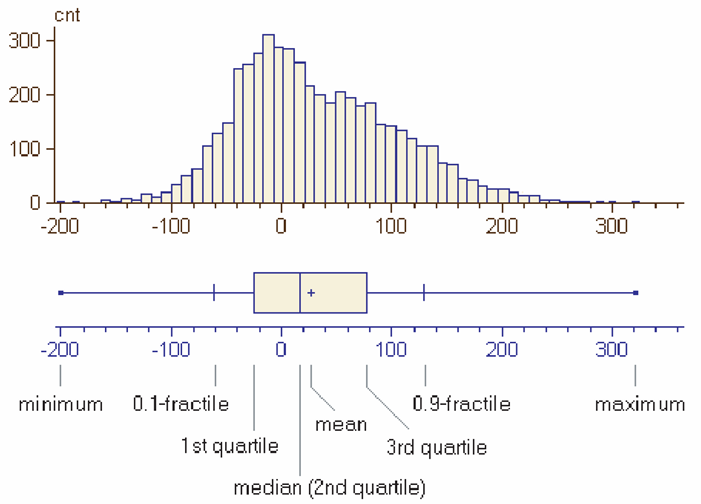
\includegraphics[width=0.7\linewidth,height=\textheight,keepaspectratio]{figs/ch3/boxplot.png}

}

\caption{\label{fig-boxplot}A box-plot example}

\end{figure}%

A \textbf{percentile} refers to the percentage of observations lying
below a given value.

A unique maximum corresponds to the \textbf{100th percentile}, while a
unique minimum corresponds to the \textbf{0th percentile}.

It follows that the \textbf{median} is the \textbf{50th percentile}. The
\textbf{25th percentile} and \textbf{75th percentile} are known as the
\textbf{first quartile} and \textbf{third quartile}, respectively.

\begin{tcolorbox}[enhanced jigsaw, coltitle=black, colbacktitle=quarto-callout-important-color!10!white, left=2mm, bottomrule=.15mm, bottomtitle=1mm, colback=white, titlerule=0mm, colframe=quarto-callout-important-color-frame, breakable, leftrule=.75mm, toptitle=1mm, opacitybacktitle=0.6, rightrule=.15mm, title=\textcolor{quarto-callout-important-color}{\faExclamation}\hspace{0.5em}{Key idea}, arc=.35mm, opacityback=0, toprule=.15mm]

Measures of relative standing tell us \emph{where} an observation lies
within a distribution, not just its magnitude.

\end{tcolorbox}

\begin{tcolorbox}[enhanced jigsaw, coltitle=black, colbacktitle=quarto-callout-important-color!10!white, left=2mm, bottomrule=.15mm, bottomtitle=1mm, colback=white, titlerule=0mm, colframe=quarto-callout-important-color-frame, breakable, leftrule=.75mm, toptitle=1mm, opacitybacktitle=0.6, rightrule=.15mm, title=\textcolor{quarto-callout-important-color}{\faExclamation}\hspace{0.5em}{Chapter summary}, arc=.35mm, opacityback=0, toprule=.15mm]

Numerical summaries allow us to describe key features of a dataset using
a small number of carefully chosen statistics.

Measures of \textbf{central location} describe where the data are
centered, while measures of \textbf{dispersion} describe how spread out
the observations are. Measures of \textbf{relative standing} indicate
how individual observations compare with the rest of the data.

Together, these tools form the foundation for understanding data and
prepare us for statistical inference in later chapters.

\end{tcolorbox}

\begin{center}\rule{0.5\linewidth}{0.5pt}\end{center}

\section{Exercises}\label{exercises-1}

\subsection{Conceptual questions}\label{conceptual-questions-1}

\begin{enumerate}
\def\labelenumi{\arabic{enumi}.}
\item
  Explain why the mean alone is often insufficient to describe a
  dataset.
\item
  Compare the mean, median, and mode.\\
  In what situations might one be preferred over the others?
\item
  Why is the median often a better measure of central location than the
  mean when data contain extreme values?
\item
  Explain why two datasets can have the same mean but very different
  standard deviations.
\end{enumerate}

\begin{tcolorbox}[enhanced jigsaw, coltitle=black, colbacktitle=quarto-callout-note-color!10!white, left=2mm, bottomrule=.15mm, bottomtitle=1mm, colback=white, titlerule=0mm, colframe=quarto-callout-note-color-frame, breakable, leftrule=.75mm, toptitle=1mm, opacitybacktitle=0.6, rightrule=.15mm, title=\textcolor{quarto-callout-note-color}{\faInfo}\hspace{0.5em}{Check your understanding}, arc=.35mm, opacityback=0, toprule=.15mm]

If two datasets have the same mean and median, must they have the same
standard deviation? Explain.

\end{tcolorbox}

\begin{center}\rule{0.5\linewidth}{0.5pt}\end{center}

\subsection{Understanding dispersion}\label{understanding-dispersion}

\begin{enumerate}
\def\labelenumi{\arabic{enumi}.}
\setcounter{enumi}{4}
\item
  Describe in words what the standard deviation measures.\\
  Why is it based on deviations from the mean rather than deviations
  from the median?
\item
  Explain the role of the root mean square (r.m.s.) in defining the
  standard deviation.
\item
  Which has larger r.m.s? the list \(7,7,7,7\) or \(7,-7,7,-7\)?
\item
  What is the r.m.s of \(17,17,17,17,17\)? What is the SD?
\item
  Can the SD ever be negative?
\item
  For a list of positive numbers, can the SD ever be larger than the
  average?
\item
  Why does the variance have squared units, and why can this make
  interpretation difficult?
\end{enumerate}

\begin{tcolorbox}[enhanced jigsaw, coltitle=black, colbacktitle=quarto-callout-warning-color!10!white, left=2mm, bottomrule=.15mm, bottomtitle=1mm, colback=white, titlerule=0mm, colframe=quarto-callout-warning-color-frame, breakable, leftrule=.75mm, toptitle=1mm, opacitybacktitle=0.6, rightrule=.15mm, title=\textcolor{quarto-callout-warning-color}{\faExclamationTriangle}\hspace{0.5em}{Common pitfall}, arc=.35mm, opacityback=0, toprule=.15mm]

A small standard deviation does not imply that the data are
``small''---only that they are tightly clustered around the mean.

\end{tcolorbox}

\begin{center}\rule{0.5\linewidth}{0.5pt}\end{center}

\subsection{Measures of relative
standing}\label{measures-of-relative-standing-1}

\begin{enumerate}
\def\labelenumi{\arabic{enumi}.}
\setcounter{enumi}{11}
\item
  Explain what it means for a value to be at the 75th percentile of a
  distribution.
\item
  Why is the median equal to the 50th percentile?
\item
  Describe how a box plot summarizes information about central location,
  dispersion, and relative standing.
\end{enumerate}

\begin{center}\rule{0.5\linewidth}{0.5pt}\end{center}

\subsection{Numerical practice}\label{numerical-practice}

\begin{enumerate}
\def\labelenumi{\arabic{enumi}.}
\setcounter{enumi}{14}
\tightlist
\item
  Consider the dataset: \[
  5,\; 8,\; 2,\; 9,\; 5,\; 3,\; 7,\; 4,\; 2,\; 7,\; 4,\; 10,\; 4,\; 3,\; 5.
  \]
\end{enumerate}

\begin{enumerate}
\def\labelenumi{\alph{enumi}.}
\tightlist
\item
  Compute the mean, median, and mode.\\
\item
  Compute the standard deviation, SD and variance.\\
\item
  Explain what each statistic tells you about the data.\\
\item
  Calculate their 25th and 75th percentiles.\\
\item
  Find the inter-quartile range (IQR).\\
\item
  Calculate the coefficient of variation for the two lists.\\
\item
  What is the mean absolute deviation for both lists?\\
\item
  Draw a boxplot for the lists of numbers.
\end{enumerate}

\begin{center}\rule{0.5\linewidth}{0.5pt}\end{center}

\subsection{Optional challenge}\label{optional-challenge-1}

\begin{enumerate}
\def\labelenumi{\arabic{enumi}.}
\setcounter{enumi}{15}
\tightlist
\item
  Find a real dataset (for example, income, test scores, or prices):
\end{enumerate}

\begin{itemize}
\tightlist
\item
  compute at least two measures of central location,
\item
  compute at least one measure of dispersion,
\item
  explain which statistics are most informative and why.
\end{itemize}

\bookmarksetup{startatroot}

\chapter{Correlation}\label{ch4}

\begin{tcolorbox}[enhanced jigsaw, coltitle=black, colbacktitle=quarto-callout-note-color!10!white, left=2mm, bottomrule=.15mm, bottomtitle=1mm, colback=white, titlerule=0mm, colframe=quarto-callout-note-color-frame, breakable, leftrule=.75mm, toptitle=1mm, opacitybacktitle=0.6, rightrule=.15mm, title=\textcolor{quarto-callout-note-color}{\faInfo}\hspace{0.5em}{Learning objectives}, arc=.35mm, opacityback=0, toprule=.15mm]

By the end of this chapter, you should be able to:

\begin{itemize}
\tightlist
\item
  distinguish between univariate and bivariate data,
\item
  use graphical tools to describe relationships between two variables,
\item
  explain why means and standard deviations are insufficient for
  describing association,
\item
  define and interpret the correlation coefficient,
\item
  compute correlation using standard units,
\item
  understand the limitations of correlation, especially with respect to
  causation.
\end{itemize}

\end{tcolorbox}

\section{Graphical representation}\label{graphical-representation}

So far, we have focused on a single variable---what is known as
\textbf{univariate data}---and examined their graphical and numerical
summaries. We now turn to \textbf{bivariate data}, that is, data
involving two variables.

As economists, we are often interested in understanding relationships
between variables---for example, wages and education, CEO performance
and salaries, economic growth and foreign aid, and many others. As with
univariate data, both \textbf{graphical} and \textbf{numerical}
summaries can be used.

\begin{tcolorbox}[enhanced jigsaw, coltitle=black, colbacktitle=quarto-callout-note-color!10!white, left=2mm, bottomrule=.15mm, bottomtitle=1mm, colback=white, titlerule=0mm, colframe=quarto-callout-note-color-frame, breakable, leftrule=.75mm, toptitle=1mm, opacitybacktitle=0.6, rightrule=.15mm, title=\textcolor{quarto-callout-note-color}{\faInfo}\hspace{0.5em}{Key graphical tools for two variables}, arc=.35mm, opacityback=0, toprule=.15mm]

The two most important graphical summaries for bivariate data are:

\begin{itemize}
\tightlist
\item
  \textbf{Contingency tables}, usually for categorical variables\\
\item
  \textbf{Scatter diagrams}, usually for quantitative variables
\end{itemize}

\end{tcolorbox}

A \textbf{contingency table} lists the frequency of each combination of
values of two categorical variables. For example, a survey of 2,237
people recording gender and handedness might produce the following
table.\footnote{For more on the relationship between categorical
  variables, a useful text is Utts and Heckard (2006, Chapter6).}

\begin{longtable}[]{@{}lll@{}}
\caption{Gender and handedness}\label{tbl-income}\tabularnewline
\toprule\noalign{}
& Male & Female \\
\midrule\noalign{}
\endfirsthead
\toprule\noalign{}
& Male & Female \\
\midrule\noalign{}
\endhead
\bottomrule\noalign{}
\endlastfoot
Right-handed & 934 & 1070 \\
Left-handed & 113 & 92 \\
Ambidextrous & 20 & 8 \\
\end{longtable}

When dealing with \textbf{cardinal (quantitative) data}, the
relationship between two variables is better visualized using a
\textbf{scatter diagram}. The figure below shows the association between
the duration of eruptions of Old Faithful and the waiting time between
eruptions.

\begin{figure}

\centering{

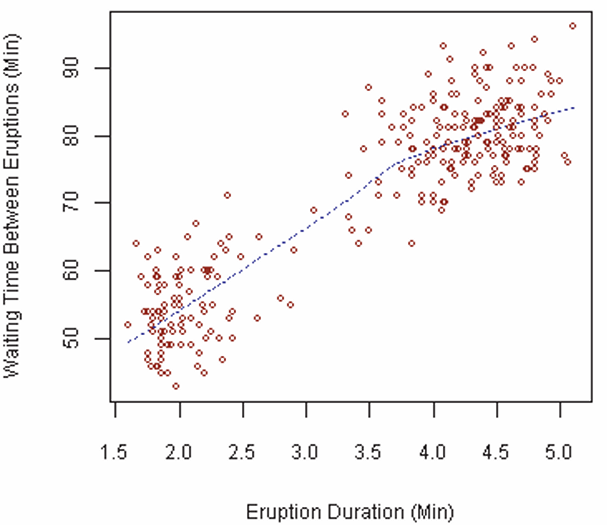
\includegraphics[width=0.7\linewidth,height=\textheight,keepaspectratio]{figs/ch4/scatter_1.png}

}

\caption{\label{fig-oldfaithful}Waiting time and eruption duration of
Old Faithful}

\end{figure}%

\section{Correlation}\label{correlation}

Graphs are informative, but they also have limitations. For this reason,
we need \textbf{numerical summaries} that describe the relationship
between two variables.

In earlier chapters, we introduced the \textbf{mean} and
\textbf{standard deviation} as the most important numerical summaries
for univariate data. One might therefore ask: \emph{Why are these not
sufficient for bivariate data?}

\begin{tcolorbox}[enhanced jigsaw, coltitle=black, colbacktitle=quarto-callout-important-color!10!white, left=2mm, bottomrule=.15mm, bottomtitle=1mm, colback=white, titlerule=0mm, colframe=quarto-callout-important-color-frame, breakable, leftrule=.75mm, toptitle=1mm, opacitybacktitle=0.6, rightrule=.15mm, title=\textcolor{quarto-callout-important-color}{\faExclamation}\hspace{0.5em}{Why means and SDs are not enough}, arc=.35mm, opacityback=0, toprule=.15mm]

Two datasets can have the same mean and standard deviation for each
variable, yet exhibit very different relationships between those
variables.

\end{tcolorbox}

Consider a university that has offered two statistics sections, \(A\)
and \(B\), over several years. For each student, midterm and final exam
scores (out of 200) are recorded and plotted.

\begin{figure}

\centering{

\pandocbounded{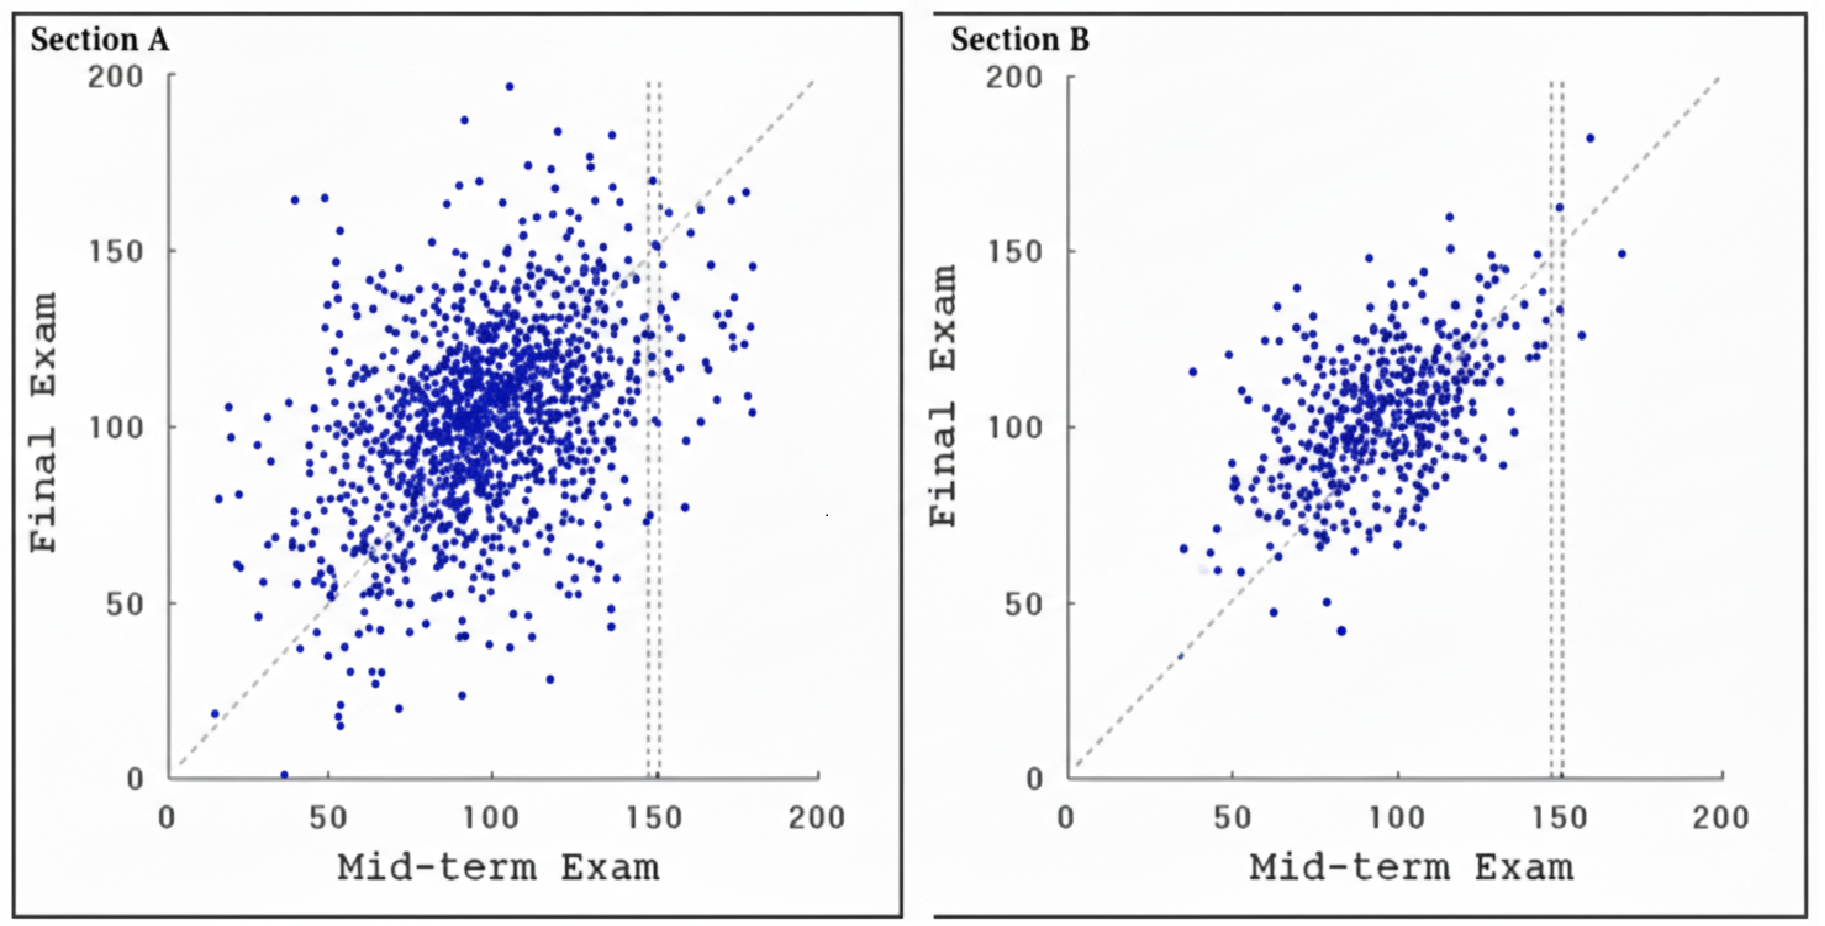
\includegraphics[keepaspectratio]{figs/ch4/scatter-ab.png}}

}

\caption{\label{fig-scatterscores}Students' score: Section A and B}

\end{figure}%

Points lying on the 45\(^\circ\) line represent students whose midterm
and final scores are the same.

If there is a \textbf{strong association}, knowing one variable helps
predict the other. If the association is weak, knowing one variable
provides little predictive power.

For example, a student in section \(A\) who scored 150 on the midterm
could plausibly score anywhere between 60 and 160 on the final. In
section \(B\), a student with the same midterm score would likely score
between 100 and 160. Midterm scores therefore provide better predictive
information in section \(B\).

More strikingly, the \textbf{means} and \textbf{standard deviations} of
both midterm and final scores are almost identical across the two
sections. This means that we cannot distinguish the sections using only
these summaries.

\begin{tcolorbox}[enhanced jigsaw, coltitle=black, colbacktitle=quarto-callout-important-color!10!white, left=2mm, bottomrule=.15mm, bottomtitle=1mm, colback=white, titlerule=0mm, colframe=quarto-callout-important-color-frame, breakable, leftrule=.75mm, toptitle=1mm, opacitybacktitle=0.6, rightrule=.15mm, title=\textcolor{quarto-callout-important-color}{\faExclamation}\hspace{0.5em}{We need a new measure}, arc=.35mm, opacityback=0, toprule=.15mm]

To capture how tightly points cluster around a line in a scatter
diagram, we introduce the \textbf{correlation coefficient}, denoted by
\(r\).

\end{tcolorbox}

\section{Correlation coefficient}\label{correlation-coefficient}

The \textbf{correlation coefficient} is a pure number between \(-1\) and
\(1\).

\begin{tcolorbox}[enhanced jigsaw, coltitle=black, colbacktitle=quarto-callout-important-color!10!white, left=2mm, bottomrule=.15mm, bottomtitle=1mm, colback=white, titlerule=0mm, colframe=quarto-callout-important-color-frame, breakable, leftrule=.75mm, toptitle=1mm, opacitybacktitle=0.6, rightrule=.15mm, title=\textcolor{quarto-callout-important-color}{\faExclamation}\hspace{0.5em}{Important}, arc=.35mm, opacityback=0, toprule=.15mm]

\[
-1 \leq Corr(X,Y) \leq 1
\]

\end{tcolorbox}

Furthermore:

\begin{itemize}
\tightlist
\item
  \(r = 1\) or \(r = -1\) indicates \textbf{perfect correlation}
\item
  A positive value of \(r\) indicates a \textbf{positive relationship}
\item
  A negative value of \(r\) indicates a \textbf{negative relationship}
\end{itemize}

The figures below show two variables with the same mean (3) and standard
deviation (1), but different correlations.

\begin{figure}

\centering{

\pandocbounded{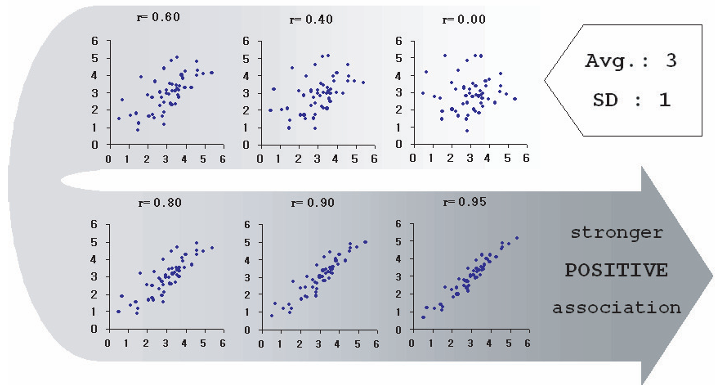
\includegraphics[keepaspectratio]{figs/ch4/positive-r.png}}

}

\caption{\label{fig-positive-corr}Positive correlation}

\end{figure}%

\begin{figure}

\centering{

\pandocbounded{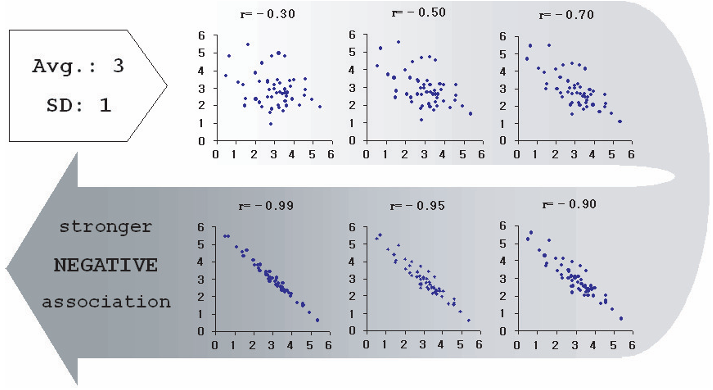
\includegraphics[keepaspectratio]{figs/ch4/negative-r.png}}

}

\caption{\label{fig-negative-corr}Negative correlation}

\end{figure}%

\begin{tcolorbox}[enhanced jigsaw, coltitle=black, colbacktitle=quarto-callout-note-color!10!white, left=2mm, bottomrule=.15mm, bottomtitle=1mm, colback=white, titlerule=0mm, colframe=quarto-callout-note-color-frame, breakable, leftrule=.75mm, toptitle=1mm, opacitybacktitle=0.6, rightrule=.15mm, title=\textcolor{quarto-callout-note-color}{\faInfo}\hspace{0.5em}{A technical detail}, arc=.35mm, opacityback=0, toprule=.15mm]

If either variable has a standard deviation equal to zero, then
\(r = 0\). Correlation requires variation in \emph{both} variables.

\end{tcolorbox}

\subsection{How correlation is
computed}\label{how-correlation-is-computed}

To compute the correlation coefficient:

\begin{enumerate}
\def\labelenumi{\arabic{enumi}.}
\tightlist
\item
  Convert each variable into \textbf{standard units}
\item
  Multiply the standard units pairwise
\item
  Take the \textbf{average} of these products
\end{enumerate}

Standard units measure distance from the mean in terms of standard
deviations.

For the list \(1, 3, 4, 5, 7\), the mean is 4 and the standard deviation
is 2. The values in standard units are:
\(-1.5,\; -0.5,\; 0,\; 0.5,\; 1.5\)

\begin{tcolorbox}[enhanced jigsaw, coltitle=black, colbacktitle=quarto-callout-important-color!10!white, left=2mm, bottomrule=.15mm, bottomtitle=1mm, colback=white, titlerule=0mm, colframe=quarto-callout-important-color-frame, breakable, leftrule=.75mm, toptitle=1mm, opacitybacktitle=0.6, rightrule=.15mm, title=\textcolor{quarto-callout-important-color}{\faExclamation}\hspace{0.5em}{Standard units}, arc=.35mm, opacityback=0, toprule=.15mm]

Standard units measure how far a value lies from the mean relative to
the spread of the data.

\end{tcolorbox}

Now consider the five points: \((1,5), (3,9), (4,7), (5,1), (7,13)\).

The mean of \(X\) is 4 with \(SD_X = 2\), and the mean of \(Y\) is 7
with \(SD_Y = 4\).

\begin{longtable}[]{@{}lllll@{}}
\caption{Calculating the correlation
coefficient}\label{tbl-calculating-corr}\tabularnewline
\toprule\noalign{}
X & Y & \(SU_X\) & \(SU_Y\) & Product \\
\midrule\noalign{}
\endfirsthead
\toprule\noalign{}
X & Y & \(SU_X\) & \(SU_Y\) & Product \\
\midrule\noalign{}
\endhead
\bottomrule\noalign{}
\endlastfoot
1 & 5 & -1.5 & -0.5 & 0.75 \\
3 & 9 & -0.5 & 0.5 & -0.25 \\
4 & 7 & 0.0 & 0.0 & 0.0 \\
5 & 1 & 0.5 & -1.5 & -0.75 \\
7 & 13 & 1.5 & 1.5 & 2.25 \\
\end{longtable}

The correlation coefficient is the \textbf{average of the last column},
which equals \(r = 0.4\).

\subsection{Why this method matters}\label{why-this-method-matters}

This approach shows that correlation:

\begin{itemize}
\tightlist
\item
  has \textbf{no units}
\item
  is unchanged by rescaling variables
\item
  measures \textbf{relative}, not absolute, clustering
\end{itemize}

There are many other ways to compute the correlation coefficient, but we
will stick to the above method as it reveals best how the correlation
coefficient works.

In many textbooks, the formula for correlation is written as:

\begin{tcolorbox}[enhanced jigsaw, coltitle=black, colbacktitle=quarto-callout-important-color!10!white, left=2mm, bottomrule=.15mm, bottomtitle=1mm, colback=white, titlerule=0mm, colframe=quarto-callout-important-color-frame, breakable, leftrule=.75mm, toptitle=1mm, opacitybacktitle=0.6, rightrule=.15mm, title=\textcolor{quarto-callout-important-color}{\faExclamation}\hspace{0.5em}{Correlation coefficient}, arc=.35mm, opacityback=0, toprule=.15mm]

\[
Corr(X,Y) = \frac{\sum_{i=1}^{n} (X_i - \overline{X})(Y_i - \overline{Y})}{\sqrt{\sum_{i=1}^{n} (X_i - \overline{X})^2} \sqrt{\sum_{i=1}^{n} (Y_i - \overline{Y})^2}}
\]

Another definition commonly used is:

\[
Corr(X,Y) = \displaystyle \frac{\text{Covariance}(X,Y)}{SD_x SD_y}
\]

\end{tcolorbox}

\begin{tcolorbox}[enhanced jigsaw, coltitle=black, colbacktitle=quarto-callout-tip-color!10!white, left=2mm, bottomrule=.15mm, bottomtitle=1mm, colback=white, titlerule=0mm, colframe=quarto-callout-tip-color-frame, breakable, leftrule=.75mm, toptitle=1mm, opacitybacktitle=0.6, rightrule=.15mm, title=\textcolor{quarto-callout-tip-color}{\faLightbulb}\hspace{0.5em}{Exercise: Correlation coefficients}, arc=.35mm, opacityback=0, toprule=.15mm]

Compute the \textbf{correlation coefficient} for each of the following
datasets.

\textbf{(a)}

\begin{longtable}[]{@{}cllllllllll@{}}
\toprule\noalign{}
\(X\) & 1 & 1 & 1 & 1 & 2 & 2 & 2 & 3 & 3 & 4 \\
\midrule\noalign{}
\endhead
\bottomrule\noalign{}
\endlastfoot
\(Y\) & 5 & 3 & 5 & 7 & 3 & 3 & 1 & 1 & 1 & 1 \\
\end{longtable}

\textbf{(b)}

\begin{longtable}[]{@{}cllllllllll@{}}
\toprule\noalign{}
\(X\) & 1 & 1 & 1 & 1 & 2 & 2 & 2 & 3 & 3 & 4 \\
\midrule\noalign{}
\endhead
\bottomrule\noalign{}
\endlastfoot
\(Y\) & 1 & 2 & 1 & 3 & 1 & 4 & 1 & 2 & 2 & 3 \\
\end{longtable}

\textbf{(c)}

\begin{longtable}[]{@{}cllllllllll@{}}
\toprule\noalign{}
\(X\) & 1 & 1 & 1 & 1 & 2 & 2 & 2 & 3 & 3 & 4 \\
\midrule\noalign{}
\endhead
\bottomrule\noalign{}
\endlastfoot
\(Y\) & 2 & 2 & 2 & 2 & 4 & 4 & 4 & 6 & 6 & 8 \\
\end{longtable}

\textbf{Question.}\\
What do you observe about the values of the correlation coefficients
across the three cases?

\end{tcolorbox}

Note that the correlation coefficient is a pure number without any
units, which is noted by the conversion to standard units.

Moreover, the correlation coefficient is *not** affected by any of the
three changes: - 1) interchanging the two variables, - 2) adding the
same number to all the values of one variable, and - 3) multiplying all
the values of one variable by the same positive number.

This basically means that changing the scale of any of the variables
leaves the correlation coefficient unchanged.

\begin{center}
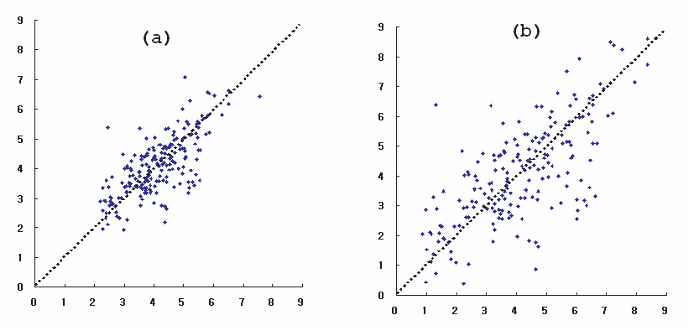
\includegraphics[width=0.8\linewidth,height=\textheight,keepaspectratio]{figs/ch4/corr-mag.png}
\end{center}

Be warned, looks can be deceiving. A quick glance at the above scatter
plots would easily convince someone that the points in (a) is more
tightly clustered, and thus having a correlation coefficient closer to
1, than (b). This cannot be further than the truth, because in fact =
0.7 for both diagrams. (b) is simply a magnification of (a). What is
important to realize is that calculating involves converting variables
to standard units (deviation from average divided by SD) and therefore
it measures clustering not in absolute terms, but in relative terms
(more specifically, relative to their standard deviations). That is,
although plot (a) may appear more tightly clustered than plot (b), both
have \(r = 0.7\). Plot (b) is simply a magnified version of plot (a).
Correlation measures clustering \textbf{relative to standard deviation},
not in absolute terms.

\begin{tcolorbox}[enhanced jigsaw, coltitle=black, colbacktitle=quarto-callout-warning-color!10!white, left=2mm, bottomrule=.15mm, bottomtitle=1mm, colback=white, titlerule=0mm, colframe=quarto-callout-warning-color-frame, breakable, leftrule=.75mm, toptitle=1mm, opacitybacktitle=0.6, rightrule=.15mm, title=\textcolor{quarto-callout-warning-color}{\faExclamationTriangle}\hspace{0.5em}{Correlation measures linear association}, arc=.35mm, opacityback=0, toprule=.15mm]

The correlation coefficient captures \textbf{linear relationships only}.
Nonlinear relationships may have low correlation even when variables are
strongly related.

\end{tcolorbox}

\section{Association is not
causation}\label{association-is-not-causation}

The last piece of warning when using correlation coefficients is to
realize that what we have is a representation of association, that is
how the variables move relative to each other. The correlation
coefficient does not establish causation. This is best left to economic
theory, which is called upon to interpret and explain the data.

\begin{tcolorbox}[enhanced jigsaw, coltitle=black, colbacktitle=quarto-callout-important-color!10!white, left=2mm, bottomrule=.15mm, bottomtitle=1mm, colback=white, titlerule=0mm, colframe=quarto-callout-important-color-frame, breakable, leftrule=.75mm, toptitle=1mm, opacitybacktitle=0.6, rightrule=.15mm, title=\textcolor{quarto-callout-important-color}{\faExclamation}\hspace{0.5em}{Important}, arc=.35mm, opacityback=0, toprule=.15mm]

Correlation measures \textbf{association}, not \textbf{causation}.

\end{tcolorbox}

A positive or negative correlation does not explain \emph{why} variables
move together. Establishing causation requires economic theory and
careful empirical reasoning.

For example, education is often thought to cause higher wages because
more educated individuals tend to earn more. However, a third
factor---such as \textbf{individual determination or motivation}---may
influence both education and wages.

Such a factor is known as a \textbf{confounding variable}, and its
presence can invalidate causal interpretations based solely on
correlation.

\begin{tcolorbox}[enhanced jigsaw, coltitle=black, colbacktitle=quarto-callout-important-color!10!white, left=2mm, bottomrule=.15mm, bottomtitle=1mm, colback=white, titlerule=0mm, colframe=quarto-callout-important-color-frame, breakable, leftrule=.75mm, toptitle=1mm, opacitybacktitle=0.6, rightrule=.15mm, title=\textcolor{quarto-callout-important-color}{\faExclamation}\hspace{0.5em}{Takeaway}, arc=.35mm, opacityback=0, toprule=.15mm]

Correlation is a powerful descriptive tool, but causal claims require
much more than a high value of \(r\).

\end{tcolorbox}

\begin{tcolorbox}[enhanced jigsaw, coltitle=black, colbacktitle=quarto-callout-important-color!10!white, left=2mm, bottomrule=.15mm, bottomtitle=1mm, colback=white, titlerule=0mm, colframe=quarto-callout-important-color-frame, breakable, leftrule=.75mm, toptitle=1mm, opacitybacktitle=0.6, rightrule=.15mm, title=\textcolor{quarto-callout-important-color}{\faExclamation}\hspace{0.5em}{Chapter summary}, arc=.35mm, opacityback=0, toprule=.15mm]

Correlation provides a numerical summary of the strength and direction
of linear association between two variables.

Scatter diagrams help visualize relationships, while the correlation
coefficient measures how tightly points cluster around a straight line.
However, correlation alone cannot establish causation, and careful
reasoning is required to interpret empirical relationships correctly.

\end{tcolorbox}

\begin{center}\rule{0.5\linewidth}{0.5pt}\end{center}

\section{Exercises}\label{exercises-2}

\subsection{Conceptual questions}\label{conceptual-questions-2}

\begin{enumerate}
\def\labelenumi{\arabic{enumi}.}
\item
  Explain the difference between univariate and bivariate data.
\item
  Why are scatter diagrams useful for studying relationships between
  quantitative variables?
\item
  Explain why two datasets can have identical means and standard
  deviations but very different correlations.
\end{enumerate}

\begin{center}\rule{0.5\linewidth}{0.5pt}\end{center}

\subsection{Understanding correlation}\label{understanding-correlation}

\begin{enumerate}
\def\labelenumi{\arabic{enumi}.}
\setcounter{enumi}{3}
\item
  What does the sign of the correlation coefficient indicate?
\item
  What does the magnitude of the correlation coefficient tell us?
\item
  Why must both variables exhibit variation for correlation to be
  meaningful?
\end{enumerate}

\begin{tcolorbox}[enhanced jigsaw, coltitle=black, colbacktitle=quarto-callout-warning-color!10!white, left=2mm, bottomrule=.15mm, bottomtitle=1mm, colback=white, titlerule=0mm, colframe=quarto-callout-warning-color-frame, breakable, leftrule=.75mm, toptitle=1mm, opacitybacktitle=0.6, rightrule=.15mm, title=\textcolor{quarto-callout-warning-color}{\faExclamationTriangle}\hspace{0.5em}{Common pitfall}, arc=.35mm, opacityback=0, toprule=.15mm]

A high correlation does not imply a causal relationship.

\end{tcolorbox}

\begin{center}\rule{0.5\linewidth}{0.5pt}\end{center}

\subsection{Computation and
interpretation}\label{computation-and-interpretation}

\begin{enumerate}
\def\labelenumi{\arabic{enumi}.}
\setcounter{enumi}{6}
\item
  Explain how converting variables to standard units removes units from
  the correlation coefficient.
\item
  Why is correlation unaffected by changes in scale or units?
\item
  Give an example of a nonlinear relationship that might have low
  correlation.
\end{enumerate}

\begin{center}\rule{0.5\linewidth}{0.5pt}\end{center}

\subsection{Optional challenge}\label{optional-challenge-2}

\begin{enumerate}
\def\labelenumi{\arabic{enumi}.}
\setcounter{enumi}{9}
\tightlist
\item
  Find two real-world variables that are correlated.\\
  Discuss whether the relationship is likely causal, and identify
  possible confounding variables.
\end{enumerate}

\bookmarksetup{startatroot}

\chapter{Elementary Probability}\label{ch7}

\begin{tcolorbox}[enhanced jigsaw, coltitle=black, colbacktitle=quarto-callout-note-color!10!white, left=2mm, bottomrule=.15mm, bottomtitle=1mm, colback=white, titlerule=0mm, colframe=quarto-callout-note-color-frame, breakable, leftrule=.75mm, toptitle=1mm, opacitybacktitle=0.6, rightrule=.15mm, title=\textcolor{quarto-callout-note-color}{\faInfo}\hspace{0.5em}{Learning objectives}, arc=.35mm, opacityback=0, toprule=.15mm]

By the end of this chapter, you should be able to:

\begin{itemize}
\tightlist
\item
  explain the main interpretations of probability,
\item
  define experiments, outcomes, sample spaces, and events,
\item
  compute conditional probabilities,
\item
  apply the multiplication and addition rules,
\item
  distinguish between independence and dependence,
\item
  understand concept of mutually exclusive,
\item
  use Bayes' rule to update probabilities,
\item
  understand the axioms underlying probability theory.
\end{itemize}

\end{tcolorbox}

In this chapter, we introduce the basic ideas of \textbf{probability}
needed to understand statistical concepts and reasoning. The literature
typically identifies \textbf{three definitions of probability}:

\begin{enumerate}
\def\labelenumi{\arabic{enumi}.}
\tightlist
\item
  the \textbf{classical} definition,\\
\item
  the \textbf{empirical (frequentist)} definition, and\\
\item
  the \textbf{subjective} definition.
\end{enumerate}

The \textbf{classical definition} assumes that all outcomes of an
experiment are equally likely. For example, when rolling a fair die, the
probability of obtaining an even number is the ratio of favorable
outcomes (2, 4, 6) to total possible outcomes (1--6), which is
\(3/6 = 1/2\).

The \textbf{empirical (frequentist) definition} is based on observed
relative frequencies. For example, one might talk about the probability
that Manchester United beats Chelsea, based on the fraction of past
games won by Manchester United.

The \textbf{subjective definition} reflects an individual's beliefs,
informed by experience and available information. For instance, a
student may assign a subjective probability to the event that they will
earn an A in a statistics course like this one.

\begin{tcolorbox}[enhanced jigsaw, coltitle=black, colbacktitle=quarto-callout-note-color!10!white, left=2mm, bottomrule=.15mm, bottomtitle=1mm, colback=white, titlerule=0mm, colframe=quarto-callout-note-color-frame, breakable, leftrule=.75mm, toptitle=1mm, opacitybacktitle=0.6, rightrule=.15mm, title=\textcolor{quarto-callout-note-color}{\faInfo}\hspace{0.5em}{A unifying point}, arc=.35mm, opacityback=0, toprule=.15mm]

Although these interpretations differ philosophically, the
\textbf{mathematics of probability} that follows does not depend on
which definition we adopt.

\end{tcolorbox}

\section{The probability space, experiment, and
outcome}\label{the-probability-space-experiment-and-outcome}

Consider tossing a coin. The outcome is uncertain: it may land
\textbf{heads} or \textbf{tails}. In probability language, tossing the
coin is an \textbf{experiment}, and the result is an \textbf{outcome}.

An experiment produces exactly \textbf{one outcome}, chosen from a set
of possible outcomes. This set is called the \textbf{sample space},
denoted \(\mathcal{S}\). A \textbf{subset} of the sample space is called
an \textbf{event}.

There is no restriction on what constitutes an experiment. Tossing one
coin once, tossing it three times, or even tossing it infinitely many
times can each be considered a single experiment.

To make this concrete, consider tossing a coin \textbf{three times}. The
sample space is

\(\mathcal{S} = \{HHH, HHT, HTH, HTT, THH, THT, TTH, TTT\}\).

If we assume each outcome is equally likely, then each has probability
\(1/8\).

\begin{tcolorbox}[enhanced jigsaw, coltitle=black, colbacktitle=quarto-callout-important-color!10!white, left=2mm, bottomrule=.15mm, bottomtitle=1mm, colback=white, titlerule=0mm, colframe=quarto-callout-important-color-frame, breakable, leftrule=.75mm, toptitle=1mm, opacitybacktitle=0.6, rightrule=.15mm, title=\textcolor{quarto-callout-important-color}{\faExclamation}\hspace{0.5em}{A basic fact}, arc=.35mm, opacityback=0, toprule=.15mm]

Probabilities always lie between 0 and 1 (or 0\% and 100\%).

More formally:

\begin{equation}\phantomsection\label{eq-probrule-1}{
0 \leq Prob(A) \leq 1
}\end{equation}

\end{tcolorbox}

From this, it follows that for any event \(A\),

\begin{equation}\phantomsection\label{eq-probrule-2}{
P(\sim A) = 1 - P(A)
}\end{equation}

where \(\sim A\) denotes the complement of \(A\) or (not A).

\section{Conditional probability}\label{conditional-probability}

Conditional probability is best understood through an example.

Suppose a deck of cards is shuffled and two cards are drawn. You win 100
baht if the \textbf{second card} is the ACE of hearts. Before seeing any
cards, the probability of winning is \(1/52\).

Now imagine that the \textbf{first card is revealed} and it is the seven
of clubs. What is your probability of winning now?

Since one card is no longer in the deck (and you know what it is), the
probability becomes \(1/51\).

Put differentlay, when pulling out two cards, because you now know the
first card, the probability of the second card is a conditional
probability i.e.~the probability of a particular event occurring, given
that another event has occurred. This is compactly written as
\(P(A \mid B)\).

\begin{tcolorbox}[enhanced jigsaw, coltitle=black, colbacktitle=quarto-callout-important-color!10!white, left=2mm, bottomrule=.15mm, bottomtitle=1mm, colback=white, titlerule=0mm, colframe=quarto-callout-important-color-frame, breakable, leftrule=.75mm, toptitle=1mm, opacitybacktitle=0.6, rightrule=.15mm, title=\textcolor{quarto-callout-important-color}{\faExclamation}\hspace{0.5em}{Conditional probability}, arc=.35mm, opacityback=0, toprule=.15mm]

Conditional probability reflects how probabilities change \textbf{once
new information becomes available}.

\end{tcolorbox}

Formally, the probability that event \(A\) occurs \textbf{given} that
event \(B\) has occurred is written

\begin{equation}\phantomsection\label{eq-conditional-prob}{
P(A \mid B)
}\end{equation}

which is read as the probability of \(A\) given \(B\).

\begin{tcolorbox}[enhanced jigsaw, coltitle=black, colbacktitle=quarto-callout-tip-color!10!white, left=2mm, bottomrule=.15mm, bottomtitle=1mm, colback=white, titlerule=0mm, colframe=quarto-callout-tip-color-frame, breakable, leftrule=.75mm, toptitle=1mm, opacitybacktitle=0.6, rightrule=.15mm, title=\textcolor{quarto-callout-tip-color}{\faLightbulb}\hspace{0.5em}{Try This: Conditional Probability}, arc=.35mm, opacityback=0, toprule=.15mm]

\textbf{(1)} Two tickets are drawn at random without replacement from
the following box:

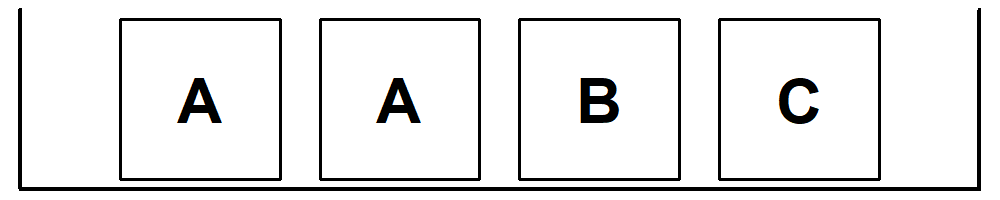
\includegraphics[width=0.4\linewidth,height=\textheight,keepaspectratio]{figs/ch7/AABC.png}

\begin{enumerate}
\def\labelenumi{(\alph{enumi})}
\tightlist
\item
  What is the chance that the second ticket is \(\fbox{B}\)?
\item
  What is the chance that the second ticket is \(\fbox{B}\), given thayt
  the fist is \(\fbox{A}\)?
\end{enumerate}

\textbf{(2)} Three cards are drawn from a deck of cards without
replacement. What is the probability that none of them will be hearts

\end{tcolorbox}

\section{The multiplication rule}\label{the-multiplication-rule}

Consider a box containing three tickets labeled R, W, and B. Two tickets
are drawn \textbf{without replacement}. What is the probability of
drawing R first and then W?

On the first draw, the probability of R is \(1/3\). Given that R was
drawn, only W and B remain, so the probability of W on the second draw
is \(1/2\). Therefore,

\(P(R \text{ then } W) = \displaystyle \frac{1}{2} \text{ of } \frac{1}{3} = \frac{1}{6}\).

This illustrates the \textbf{multiplication rule}:

\begin{equation}\phantomsection\label{eq-multiplication-rule}{
P(AB) = P(B \mid A)P(A) = P(A \mid B)P(B)
}\end{equation}

For example, the probability that \textbf{two cards dealt from a deck
are both ACES} is

\(\displaystyle \frac{3}{51} \times \frac{4}{54}\).

\section{Independence}\label{independence}

Two events are said to be \textbf{independent} if knowing the outcome of
one does not affect the probability of the other.

Drawing with replacement produces independent events; drawing without
replacement produces dependent events.

\begin{tcolorbox}[enhanced jigsaw, coltitle=black, colbacktitle=quarto-callout-important-color!10!white, left=2mm, bottomrule=.15mm, bottomtitle=1mm, colback=white, titlerule=0mm, colframe=quarto-callout-important-color-frame, breakable, leftrule=.75mm, toptitle=1mm, opacitybacktitle=0.6, rightrule=.15mm, title=\textcolor{quarto-callout-important-color}{\faExclamation}\hspace{0.5em}{Independence}, arc=.35mm, opacityback=0, toprule=.15mm]

Events A and B as said to be \textbf{independent} if

\begin{equation}\phantomsection\label{eq-independent}{
P(A \mid B) = P(A)
}\end{equation}

(or equivalently \(P(B \mid A) = P(B)\)).

\end{tcolorbox}

When we have independence, the multiplication rule conveniently
simplifies to

\begin{equation}\phantomsection\label{eq-multiplication-rule-independent}{
P(AB) = P(A)P(B)
}\end{equation}

\textbf{Try these:} \textbf{(1)} A fair coin is tossed twice. What is
the chance of getting a head then a tail? \textbf{(2)} A die is rolled
three times. (i) Find the chance that the first roll is an ACE. (ii)
Find the chance that the first roll is an ACE, the second roll is a
deuce, and the third roll is a trey..

\section{Checking for independence}\label{checking-for-independence}

Suppose we want to know whether graduating from GA program helps someone
become a successful manager/CEO.

Let:

\begin{itemize}
\tightlist
\item
  \(A_i\): GA graduate \texttt{(=1)}, or 0 otherwise\\
\item
  \(B_i\): Becomes CEO \texttt{(=1)}, or 0 otherwise
\end{itemize}

The table below summarizes survey results:

\begin{longtable}[]{@{}llll@{}}
\toprule\noalign{}
& Becomes CEO & Does not become CEO & \textbf{Total} \\
\midrule\noalign{}
\endhead
\bottomrule\noalign{}
\endlastfoot
GA graduate & 0.11 & 0.29 & 0.40 \\
Not GA graduate & 0.06 & 0.54 & 0.60 \\
\textbf{Total} & 0.17 & 0.83 & 1.00 \\
\end{longtable}

The \textbf{marginal probability} of becoming a CEO is 0.17. The
\textbf{joint probability} of a GA graduate becoming a CEO is 0.11, and
so on.

\begin{tcolorbox}[enhanced jigsaw, coltitle=black, colbacktitle=quarto-callout-important-color!10!white, left=2mm, bottomrule=.15mm, bottomtitle=1mm, colback=white, titlerule=0mm, colframe=quarto-callout-important-color-frame, breakable, leftrule=.75mm, toptitle=1mm, opacitybacktitle=0.6, rightrule=.15mm, title=\textcolor{quarto-callout-important-color}{\faExclamation}\hspace{0.5em}{Marginal probability from joint probabilities}, arc=.35mm, opacityback=0, toprule=.15mm]

To get the \emph{marginal} probability of a student being a GA graduate,
we add the two joint probabilities of the first row \((0.11 + 029)\) to
get \(0.4\). Note here the two jint probabilities that we add, the
probability that we have a GA graduate and CEO \emph{plus} the
probability that we have a GA graduate and not a CEO. Here probabilty of
GA is the same, but we have CEO and not CEO. So by adding across CEO
type, we essentially \textbf{integrate it out} and we are left with the
marginal probabilty of 0.4, the probability of GA graduate.

\end{tcolorbox}

To test independence, compute

\(P(A_1 \mid B_1) = \displaystyle \frac{P(A_1 B_1)}{P(B_1)} = \displaystyle \frac{0.11}{0.17} \approx 0.65\).

Since \(P(A_1 \mid B_1) \neq P(A_1)\), the two events are \textbf{not
independent}.

\begin{tcolorbox}[enhanced jigsaw, coltitle=black, colbacktitle=quarto-callout-tip-color!10!white, left=2mm, bottomrule=.15mm, bottomtitle=1mm, colback=white, titlerule=0mm, colframe=quarto-callout-tip-color-frame, breakable, leftrule=.75mm, toptitle=1mm, opacitybacktitle=0.6, rightrule=.15mm, title=\textcolor{quarto-callout-tip-color}{\faLightbulb}\hspace{0.5em}{Interpretation}, arc=.35mm, opacityback=0, toprule=.15mm]

Becoming a CEO is related to being a GA graduate in this example.

\end{tcolorbox}

\section{The addition rule}\label{the-addition-rule}

Two events are said to be \textbf{mutually exclusive} if the occurrence
of one prevents the occurrence of the other.

For mutually exclusive events,

\begin{equation}\phantomsection\label{eq-additional-rule-mutually-exclusive}{
P(A \text{ or } B) = P(A) + P(B)
}\end{equation}

For example, intuitively, if we draw one card from a deck of cards, the
probability of getting either a heart or spades is
\(\frac{1}{4} + \frac{1}{4} = \frac{1}{2}\). The additional rule tells
us to simply add the chances provided that the two events are mutually
exclusive. The probability to get a heart is 1/4 and the probability to
get a spade is also 1/4. Are the two events mutually exclusive? Yes,
getting a heart means you can't get a spade, and vice versa. So simply
add the chances to get \(1/4 + 1/4 = 1/2.\)

However, for events that are \textbf{not mutually exclusive}, the
general addition rule is

\begin{equation}\phantomsection\label{eq-additional-rule}{
P(A \text{ or } B) = P(A) + P(B) - P(A \text{ and } B)
}\end{equation}

For example, if we toss two dice at the same time, to get at least ace
on the two dice, we calculate the probability using the general
additional rule, i.e we add the chances and subtract the joint
probability because the two events are not mutually exclusive since
having an ace on one of the die does not exclude the possibility to get
an ace on the other die. In other words, it is possible to get ACE in
both dice, i.e.~the events are \textbf{not} mutually exclusive! Hence we
get \(1/6 + 1/6 - 1/36 = 11/36.\)

\begin{tcolorbox}[enhanced jigsaw, coltitle=black, colbacktitle=quarto-callout-important-color!10!white, left=2mm, bottomrule=.15mm, bottomtitle=1mm, colback=white, titlerule=0mm, colframe=quarto-callout-important-color-frame, breakable, leftrule=.75mm, toptitle=1mm, opacitybacktitle=0.6, rightrule=.15mm, title=\textcolor{quarto-callout-important-color}{\faExclamation}\hspace{0.5em}{Mutually exclusive events}, arc=.35mm, opacityback=0, toprule=.15mm]

Events A and B as said to be \textbf{mutually exclusive} if

\begin{equation}\phantomsection\label{eq-muutually-exclusive}{
P(A \text{ and } B) = 0
}\end{equation}

\end{tcolorbox}

Note that we have used the word `or' and `at least' for the additional
rule, which can be contrasted with `and' for the multiplication rule. In
terms of set operations, these are the union and intersect operators,
respectively.

\begin{tcolorbox}[enhanced jigsaw, coltitle=black, colbacktitle=quarto-callout-important-color!10!white, left=2mm, bottomrule=.15mm, bottomtitle=1mm, colback=white, titlerule=0mm, colframe=quarto-callout-important-color-frame, breakable, leftrule=.75mm, toptitle=1mm, opacitybacktitle=0.6, rightrule=.15mm, title=\textcolor{quarto-callout-important-color}{\faExclamation}\hspace{0.5em}{Try these.}, arc=.35mm, opacityback=0, toprule=.15mm]

\textbf{(1)} A die is rolled twice. What is (a) the chance that the
first roll is an ace or the second roll is an ace? (b) the chance that
the first roll is an ace and the second roll is an ace? (c) the cace of
getting at least one ace?

\textbf{(2)} A deck of cards is shuffled. What is (a) the chance that
the top card is an ace of spades or the bottom card is an ace of spades?
(b) the chance that the first card is an ace of spades and the bottom
card is an ace of spades?

\end{tcolorbox}

\section{Venn diagrams}\label{venn-diagrams}

Venn diagrams are very useful when thinking about simple probability
problems.\\
For example, two events A and B that are not disjoint can be drawn as
follows:

\begin{center}
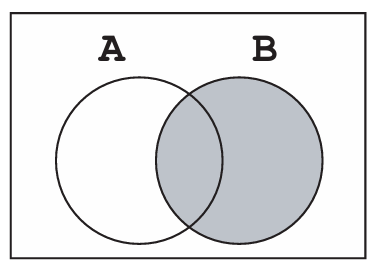
\includegraphics[width=0.4\linewidth,height=\textheight,keepaspectratio]{figs/ch7/venn-ab.png}
\end{center}

Even more useful, the conditional probability can be shown by the
following:

\(P(A|B) =\)

\pandocbounded{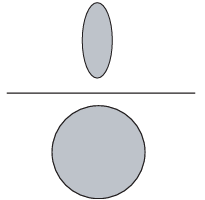
\includegraphics[keepaspectratio]{figs/ch7/venn-lc.png}}
or \(\frac{P(AB)}{P(B)}.\) That is, given B we wish to know A.

\section{Bayes' rule}\label{bayes-rule}

We can easily derive the Bayes' Rule using Venn diagrams.

Taking a sample space with event A:

\pandocbounded{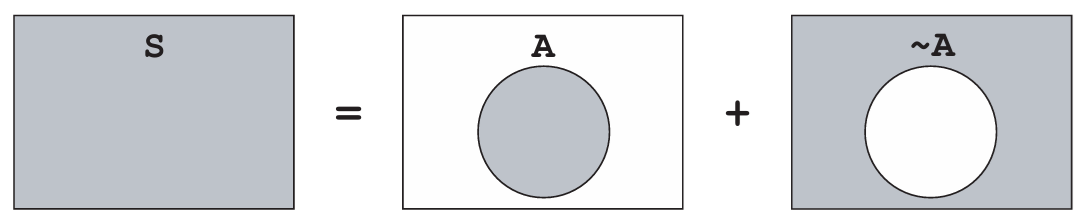
\includegraphics[keepaspectratio]{figs/ch7/bayes-1.png}}

Similarly, the probability of B can be shown using the Venn diagram as
follows: \textbackslash{}

\pandocbounded{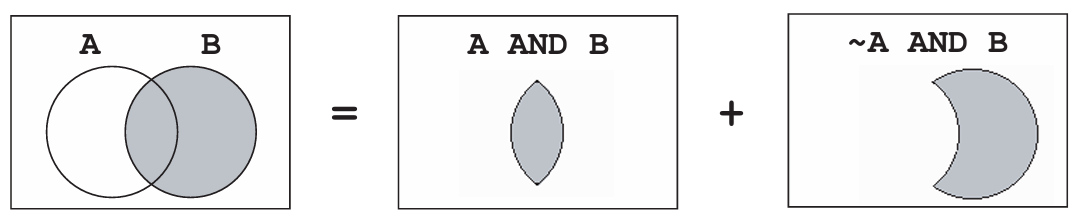
\includegraphics[keepaspectratio]{figs/ch7/bayes-2.png}}

Combining the two Venn diagrams we get:\textbackslash{}

\pandocbounded{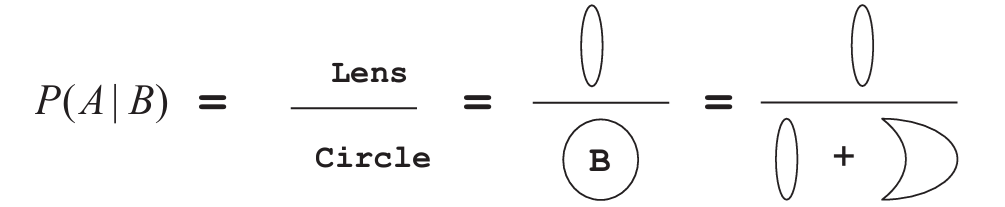
\includegraphics[keepaspectratio]{figs/ch7/bayes-3.png}}

Or what is the same thing

\[
P(A|B) = \frac {P(A \text{ and } B)}{P(B)} = \frac {P(A \text{ and } B)}{P(A \text{ and } B) + P(\sim A \text{ and } B)}
\]

And finally from the definition of joint probabilities we have the Bayes
Rule.

\begin{tcolorbox}[enhanced jigsaw, coltitle=black, colbacktitle=quarto-callout-important-color!10!white, left=2mm, bottomrule=.15mm, bottomtitle=1mm, colback=white, titlerule=0mm, colframe=quarto-callout-important-color-frame, breakable, leftrule=.75mm, toptitle=1mm, opacitybacktitle=0.6, rightrule=.15mm, title=\textcolor{quarto-callout-important-color}{\faExclamation}\hspace{0.5em}{Bayes' Rule}, arc=.35mm, opacityback=0, toprule=.15mm]

\begin{equation}\phantomsection\label{eq-bayes-rule}{
P(A \mid B) = \frac{P(A)P(B \mid A)}{P(A)P(B \mid A) + P(\sim A)P(B \mid \sim A)}
}\end{equation}

\end{tcolorbox}

So how do we use the Bayes' Rule? An example should illustrate this.
Assume that on a dark night, there was a hit and run accident. A
witness, who says that she saw a blue taxi, agrees to sit in the court
to testify for the victim so that the latter might get some compensation
from the blue taxi company. Incidentally, there are 200 taxis in this
town; 170 or 85 \% belong to the black taxi company and 30 or 15 \% are
blue. According to tests conducted under the same condition, the witness
identifies blue taxi about 80 \% of the time. Now, the question is, What
is the probability that she was right, that she really did see a blue
taxi that night?

\begin{itemize}
\tightlist
\item
  15\% of taxis are blue\\
\item
  85\% are black\\
\item
  The witness correctly identifies blue taxis 80\% of the time\\
\item
  She incorrectly identifies black taxis as blue 20\% of the time
\end{itemize}

To use Bayes' formula, all we have to identify are a few marginal and
conditional probabilities; \(P(A)\) is the probability that the taxi
involved in the accident is blue (i.e 15 \%.) Hence \(P(\sim A)\) that
is the probability of a black taxi, is 85 \%. \(P(B \mid A)\) is the
probability that the witness claims to have seen blue when a blue taxi
was really involved, in other words, her accuracy in identifying a blue
taxi correctly under the conditions. Conversely, the only other
probability we need now to complete the equation is
\(P(B \mid \sim A)\), which is the probability that the witness sees a
blue taxi when in fact a black taxi was involved. i.e 20 \%. Plugging
all the relevant probabilities gives:

\(P(A \mid B) = \displaystyle \frac{0.15 \times 0.80}{(0.15 \times 0.80) + (0.85 \times 0.20)} = \frac{0.12}{0.29} \approx 0.41\).

The probability that the witness says she saw ``blue'' and that it was
really a blue taxi is only 0.41, hardly sufficient for the courts to ask
the blue taxi company to pay compensation!\footnote{Another way to see
  this is, say we present the witness the 30 Blue taxis, she will
  identify 80\% or 24 as blue (and 6 as black) under the same night
  conditions. Also she will identify 20\% or 34 of 170 black taxis as
  `blue'. So out of 54 taxis she calls `blue', only 24 are in fact blue,
  which is about 41\%.}

\begin{tcolorbox}[enhanced jigsaw, coltitle=black, colbacktitle=quarto-callout-warning-color!10!white, left=2mm, bottomrule=.15mm, bottomtitle=1mm, colback=white, titlerule=0mm, colframe=quarto-callout-warning-color-frame, breakable, leftrule=.75mm, toptitle=1mm, opacitybacktitle=0.6, rightrule=.15mm, title=\textcolor{quarto-callout-warning-color}{\faExclamationTriangle}\hspace{0.5em}{A sobering result}, arc=.35mm, opacityback=0, toprule=.15mm]

Even confident testimony can be misleading when base rates are ignored.

\end{tcolorbox}

\begin{tcolorbox}[enhanced jigsaw, coltitle=black, colbacktitle=quarto-callout-tip-color!10!white, left=2mm, bottomrule=.15mm, bottomtitle=1mm, colback=white, titlerule=0mm, colframe=quarto-callout-tip-color-frame, breakable, leftrule=.75mm, toptitle=1mm, opacitybacktitle=0.6, rightrule=.15mm, title=\textcolor{quarto-callout-tip-color}{\faLightbulb}\hspace{0.5em}{Probability tree diagram}, arc=.35mm, opacityback=0, toprule=.15mm]

We can represent the example in a tree diagram.

\begin{Shaded}
\begin{Highlighting}[]
\NormalTok{                            Start: Taxi Accident}
\NormalTok{                                   |}
\NormalTok{               ┌───────────────────┴───────────────────┐}
\NormalTok{               │                                       │}
\NormalTok{           Blue Taxi (A)                         Black Taxi (\textasciitilde{}A)}
\NormalTok{           P(A) = 0.15                          P(\textasciitilde{}A) = 0.85}
\NormalTok{               |                                       |}
\NormalTok{        ┌──────┴───────┐                       ┌──────┴───────┐}
\NormalTok{        │              │                       │              │}
\NormalTok{  Says Blue (B)   Says Black (\textasciitilde{}B)        Says Blue (B)   Says Black (\textasciitilde{}B)}
\NormalTok{  P(B|A)=0.80     P(\textasciitilde{}B|A)=0.20          P(B|\textasciitilde{}A)=0.20     P(\textasciitilde{}B|\textasciitilde{}A)=0.80}
\NormalTok{        |              |                       |              |}
\NormalTok{        ▼              ▼                       ▼              ▼}
\NormalTok{  Joint: 0.12     Joint: 0.03           Joint: 0.17      Joint: 0.68}
\NormalTok{  P(A∩B)          P(A∩\textasciitilde{}B)               P(\textasciitilde{}A∩B)          P(\textasciitilde{}A∩\textasciitilde{}B)}
\end{Highlighting}
\end{Shaded}

We see that:

\(P(AB) = 0.12\)\\
\(P(B) = P(A∩B) + P(\sim A∩B) = 0.12 + 0.17 = 0.29\) i.e.~the marginal
probability of \(B\) by \emph{integrating out} \(A\) by summing across
\(A\). And since we are looking for \(P(A|B)\)
i.e.~\(P(AB)/P(B) ≈ 0.41\), which is the probability the taxi was blue
given that the witness says blue!

\end{tcolorbox}

\subsubsection{Bayes' Updating}\label{bayes-updating}

Essentially, we have:

\begin{center}
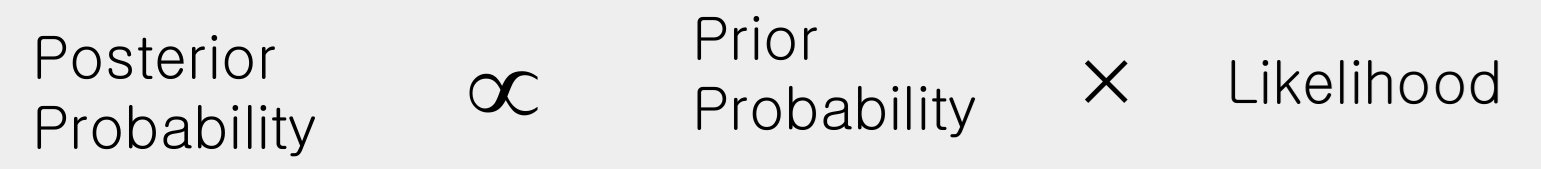
\includegraphics[width=0.7\linewidth,height=\textheight,keepaspectratio]{figs/ch7/bayes-updating.png}
\end{center}

\textbf{Prior Probability (15\%):} This represents our initial belief
about the situation before considering the witness testimony. Based on
the town's taxi distribution, we know that only 15\% of taxis are blue.
This is our baseline expectation that any random taxi involved in an
accident would be blue.

\textbf{Likelihood (Witness Accuracy):} This quantifies how probable the
observed evidence (witness testimony) is under different hypotheses. The
witness correctly identifies blue taxis 80\% of the time and incorrectly
identifies black taxis as blue 20\% of the time. This creates two
competing likelihoods: - If the taxi was actually blue, we'd expect her
to say ``blue'' 80\% of the time - If the taxi was actually black, we'd
expect her to mistakenly say ``blue'' 20\% of the time

\textbf{Posterior Probability (41\%):} This is the updated probability
that combines our prior belief with the new evidence. Using Bayes'
theorem, we find that even though the witness says she saw a blue taxi,
there's only about a 41\% chance she's actually correct. This
counterintuitive result occurs because blue taxis are rare (15\%) and
the false positives from the much more common black taxis outweigh the
true positives.

\textbf{Intuition Behind the Result:} The Bayesian approach forces us to
consider both the reliability of the evidence AND the base rates (or
prioir provbailities). Even with a seemingly reliable witness (80\%
accurate), the rarity of blue taxis means most ``blue'' identifications
will be errors. This explains why the court should be skeptical---the
witness's claim only increases the probability from 15\% to 41\%, far
from ``beyond reasonable doubt.''

\textbf{Extension: What If We Had Another Witness?} If a second
independent witness also claimed to see a blue taxi, Bayesian updating
would apply again. The first posterior (41\%) would become our new
prior, and we'd combine it with the second witness's reliability.
Intuitively, this would increase our confidence, but mathematically,
we'd need to consider (1) whether the witnesses are truly independent,
(2) whether they have the same accuracy rates, and (3) the possibility
of collusion or shared biases.

With two independent, reliable witnesses both saying ``blue,'' the
probability that the taxi was actually blue would increase
substantially, potentially making the evidence strong enough for legal
purposes. This demonstrates how Bayesian updating elegantly handles
accumulating evidence---each new piece of information updates our
beliefs in a mathematically rigorous way.

\section{Axioms of probability}\label{axioms-of-probability}

Probability rests on three axioms:

\begin{enumerate}
\def\labelenumi{\arabic{enumi}.}
\tightlist
\item
  \textbf{Nonnegativity:} \(P(A) \ge 0\)\\
\item
  \textbf{Additivity:} For disjoint events,
  \(P(A \cup B) = P(A) + P(B)\)\\
\item
  \textbf{Normalization:} \(P(\mathcal{S}) = 1\)
\end{enumerate}

From these axioms follow many useful properties, such as:

\begin{itemize}
\tightlist
\item
  If \(A \subset B\), then \(P(A) \le P(B)\)\\
\item
  \(P(A \cup B) = P(A) + P(B) - P(A \cap B)\)\\
\item
  \(P(A \cup B) \le P(A) + P(B)\)
\end{itemize}

\begin{tcolorbox}[enhanced jigsaw, coltitle=black, colbacktitle=quarto-callout-important-color!10!white, left=2mm, bottomrule=.15mm, bottomtitle=1mm, colback=white, titlerule=0mm, colframe=quarto-callout-important-color-frame, breakable, leftrule=.75mm, toptitle=1mm, opacitybacktitle=0.6, rightrule=.15mm, title=\textcolor{quarto-callout-important-color}{\faExclamation}\hspace{0.5em}{Chapter summary}, arc=.35mm, opacityback=0, toprule=.15mm]

Probability provides a formal language for reasoning under uncertainty.
In this chapter, we introduced experiments, events, conditional
probability, independence, and the fundamental rules governing
probabilities. These ideas form the foundation for statistical inference
in the chapters ahead.

\end{tcolorbox}

\begin{center}\rule{0.5\linewidth}{0.5pt}\end{center}

\section{Exercises}\label{exercises-3}

\subsection{Conceptual questions}\label{conceptual-questions-3}

\begin{enumerate}
\def\labelenumi{\arabic{enumi}.}
\item
  \textbf{Three views of probability}\\
  Explain the difference between the \textbf{classical},
  \textbf{frequentist}, and \textbf{subjective} interpretations of
  probability.\\
  Give one real-world example for each interpretation.
\item
  \textbf{Probability without philosophy}\\
  The chapter argues that the mathematics of probability does not depend
  on which interpretation we adopt.\\
  Explain what this means in your own words.
\item
  \textbf{Experiments and outcomes}\\
  Consider the experiment \emph{``toss a fair coin until a head
  appears.''}

  \begin{itemize}
  \tightlist
  \item
    What is the sample space?\\
  \item
    Is this a finite or infinite sample space?\\
  \item
    Why is this still considered a \emph{single} experiment?
  \end{itemize}
\item
  \textbf{Events vs outcomes}\\
  Explain the difference between an \textbf{outcome} and an
  \textbf{event}.\\
  Can a single outcome itself be an event?
\item
  \textbf{Conditional probability and information}\\
  Why does conditional probability capture the idea of \emph{learning
  from new information}?\\
  Give an example (not involving cards or coins) where learning new
  information changes probabilities.
\item
  \textbf{Independence vs mutual exclusivity}\\
  Are mutually exclusive events ever independent?\\
  Carefully explain your answer.
\end{enumerate}

\begin{center}\rule{0.5\linewidth}{0.5pt}\end{center}

\subsection{Basic probability
calculations}\label{basic-probability-calculations}

\begin{enumerate}
\def\labelenumi{\arabic{enumi}.}
\setcounter{enumi}{6}
\tightlist
\item
  \textbf{Coins and sample spaces}\\
  A fair coin is tossed four times.

  \begin{itemize}
  \tightlist
  \item
    How many outcomes are in the sample space?\\
  \item
    What is the probability of getting exactly two heads?\\
  \item
    What is the probability of getting at least one head?
  \end{itemize}
\item
  \textbf{Complements}\\
  Let event \(A\) be \emph{``a randomly selected student passes an
  exam''}, with \(P(A)=0.85\).

  \begin{itemize}
  \tightlist
  \item
    What is \(P(\sim A)\)?\\
  \item
    Interpret this probability in words.
  \end{itemize}
\item
  \textbf{Cards and conditional probability}\\
  A card is drawn at random from a standard deck.

  \begin{itemize}
  \tightlist
  \item
    What is the probability that it is a queen?\\
  \item
    What is the probability that it is a queen \textbf{given} that it is
    a face card?\\
  \item
    Are the events \emph{``queen''} and \emph{``face card''}
    independent?
  \end{itemize}
\end{enumerate}

\begin{center}\rule{0.5\linewidth}{0.5pt}\end{center}

\subsection{Multiplication rule and
independence}\label{multiplication-rule-and-independence}

\begin{enumerate}
\def\labelenumi{\arabic{enumi}.}
\setcounter{enumi}{9}
\item
  \textbf{Without replacement}\\
  Two cards are drawn \emph{without replacement} from a standard deck.

  \begin{itemize}
  \tightlist
  \item
    What is the probability that both cards are red?\\
  \item
    What is the probability that the first card is an ace and the second
    card is also an ace?
  \end{itemize}
\item
  \textbf{With replacement}\\
  Repeat Question 10, but now assume the first card is replaced before
  the second draw.\\
  Explain why the probabilities change.
\item
  \textbf{Testing independence}\\
  Two events satisfy

  \(P(A)=0.4\), \(P(B)=0.5\), and \(P(AB)=0.2\).

  \begin{itemize}
  \tightlist
  \item
    Are \(A\) and \(B\) independent?\\
  \item
    Justify your answer mathematically.
  \end{itemize}
\end{enumerate}

\begin{center}\rule{0.5\linewidth}{0.5pt}\end{center}

\subsection{Addition rule and mutually exclusive
events}\label{addition-rule-and-mutually-exclusive-events}

\begin{enumerate}
\def\labelenumi{\arabic{enumi}.}
\setcounter{enumi}{12}
\tightlist
\item
  \textbf{Mutually exclusive or not?}\\
  For each pair of events below, state whether they are mutually
  exclusive and explain why:

  \begin{itemize}
  \tightlist
  \item
    Drawing a heart and drawing a spade\\
  \item
    Drawing a heart and drawing a red card\\
  \item
    Getting a head on the first toss and a tail on the second toss
  \end{itemize}
\item
  \textbf{Dice example}\\
  Two fair dice are rolled.

  \begin{itemize}
  \tightlist
  \item
    What is the probability that at least one die shows a 6?\\
  \item
    Use the general addition rule to compute your answer.
  \end{itemize}
\end{enumerate}

\begin{center}\rule{0.5\linewidth}{0.5pt}\end{center}

\subsection{Bayes' rule and
interpretation}\label{bayes-rule-and-interpretation}

\begin{enumerate}
\def\labelenumi{\arabic{enumi}.}
\setcounter{enumi}{14}
\tightlist
\item
  \textbf{Medical testing}\\
  A disease affects 2\% of a population.\\
  A diagnostic test correctly identifies the disease 95\% of the time,
  but incorrectly signals disease in 5\% of healthy individuals.

  \begin{itemize}
  \tightlist
  \item
    Define the relevant events.\\
  \item
    Use Bayes' rule to compute the probability that a person who tests
    positive actually has the disease.\\
  \item
    Explain the result in words.
  \end{itemize}
\item
  \textbf{Base-rate neglect}\\
  In the taxi example discussed in the chapter, many people expect the
  probability to be close to 0.8.\\
  Explain why this intuition is misleading.
\end{enumerate}

\begin{center}\rule{0.5\linewidth}{0.5pt}\end{center}

\subsection{Set Operations and Probability
Identities}\label{set-operations-and-probability-identities}

\begin{enumerate}
\def\labelenumi{\arabic{enumi}.}
\setcounter{enumi}{16}
\tightlist
\item
  Set operations and De Morgan's laws
\end{enumerate}

\begin{enumerate}
\def\labelenumi{(\alph{enumi})}
\tightlist
\item
  Consider rolling a fair die. Let\\
\end{enumerate}

\begin{itemize}
\tightlist
\item
  \(A\) be the set of outcomes where the roll is an \textbf{even
  number}, and\\
\item
  \(B\) be the set of outcomes where the roll is \textbf{greater than
  3}.
\end{itemize}

Calculate and compare the sets on both sides of De Morgan's laws:

\[
\sim (A \cup B) = \sim A \cap \sim B
\qquad \text{and} \qquad
\sim (A \cap B) = \sim A \cup \sim B.
\]

\begin{enumerate}
\def\labelenumi{(\alph{enumi})}
\setcounter{enumi}{1}
\tightlist
\item
  Show that
\end{enumerate}

\[
\sim A = (\sim A \cap B) \cup (\sim A \cap \sim B),
\]

and

\[
\sim B = (A \cap \sim B) \cup (\sim A \cap \sim B).
\]

\begin{enumerate}
\def\labelenumi{(\alph{enumi})}
\setcounter{enumi}{2}
\tightlist
\item
  Show that
\end{enumerate}

\[
\sim (A \cap B)
= (\sim A \cap B) \cup (\sim A \cap \sim B) \cup (A \cap \sim B).
\]

\begin{enumerate}
\def\labelenumi{\arabic{enumi}.}
\setcounter{enumi}{17}
\tightlist
\item
  Probability inequality
\end{enumerate}

Prove that for any two events \(A\) and \(B\),

\[
P(A \cap B) \ge P(A) + P(B) - 1.
\]

\emph{Hint:} Use the axioms of probability and the addition rule.

\begin{enumerate}
\def\labelenumi{\arabic{enumi}.}
\setcounter{enumi}{18}
\tightlist
\item
  Law of total probability
\end{enumerate}

Show the identity

\[
P(A \mid B)
= P(C \mid B)P(A \mid B \cap C)
+ P(\sim C \mid B)P(A \mid B \cap \sim C).
\]

Explain briefly how this formula relates to conditioning on whether
event \(C\) occurs or not.

\begin{center}\rule{0.5\linewidth}{0.5pt}\end{center}

\subsection{Reflection and
interpretation}\label{reflection-and-interpretation}

\begin{enumerate}
\def\labelenumi{\arabic{enumi}.}
\setcounter{enumi}{19}
\item
  \textbf{Probability and statistical reasoning}\\
  Explain why probability theory is essential for understanding
  statistical concepts such as correlation and regression.
\item
  \textbf{From probability to inference}\\
  Which ideas from this chapter do you think will be most important when
  we later study statistical inference?\\
  Briefly explain why.
\end{enumerate}

\bookmarksetup{startatroot}

\chapter{Discrete Probability Distributions}\label{ch8}

We begin by defining a \textbf{random variable} as a function or rule
that assigns a number to each outcome of an experiment. Instead of
talking about the coin flipping event as \{heads, tails\}, for example,
we can think of it as 1 and 0, what we often call an indicator variable.
This is actually a numerical event which can be called `the number of
heads when flipping a coin'.

Formally, a random variable is defined as:

\[
X: \Omega \to \mathbb{R}
\] where \(\Omega\) is the sample space (all possible outcomes of the
experiment), \(X\) is a measurable function that maps each outcome
\(\omega \in \Omega\) to a real number \(X(\omega)\).

So, the experiment produces an outcome \(\omega\), and the random
variable translates that outcome into a number. Hence one can view the
random variables as a `bridge'\,''\,' from experiment → numbers.

The \textbf{probability distribution} is a listing of all possible
outcomes of an experiment and the corresponding probability. Once we
have a random variable \(X\), we can ask: how likely is each possible
value of \(X\)? That's where the distribution comes in. It is the
probability measure induced by \(X\):

\[
P_X(A)=P(\{\omega \in \Omega: X(\omega) \in A \})
\] where \(P\) is the probability measure on the sample space, \(P_X\)
is the distribution of \(X\) and \(A\) is a set of real numbers (e.g.,
an interval).

This tells us: the probability that \(X\) takes values in \(A\) is equal
to the probability of all outcomes that map into \(A\). In pther words,
a distribution is like a rulebook-it specifies the probabilities
attached to those numbers, telling us the `laws' governing randomness.

\subsection{Tossing a fair coin}\label{tossing-a-fair-coin}

This approach shows that correlation:

\begin{itemize}
\tightlist
\item
  Sample space: \(\Omega =\) \{Heads, Tails\}
\item
  Random variable: \(X\)(Heads) \(=1\), \(X\)(Tails) \(=0\)\\
\item
  Distribution: \(P(X=1)=1/2\), \(P(X=0)=1/2\)
\end{itemize}

A discrete distribution is based on random variables which can assume
only clearly separated values i.e.~takes on only whole numbers like
\(0, 1, 2, \dots\) while a continuous distribution can assume an
infinite number of values i.e.~takes on any value on the Real line,
within a given range. A useful analogy is ``Integers are discrete, while
Real Numbers are continuous''.

\begin{tcolorbox}[enhanced jigsaw, coltitle=black, colbacktitle=quarto-callout-important-color!10!white, left=2mm, bottomrule=.15mm, bottomtitle=1mm, colback=white, titlerule=0mm, colframe=quarto-callout-important-color-frame, breakable, leftrule=.75mm, toptitle=1mm, opacitybacktitle=0.6, rightrule=.15mm, title=\textcolor{quarto-callout-important-color}{\faExclamation}\hspace{0.5em}{Discrete vs.~Continious}, arc=.35mm, opacityback=0, toprule=.15mm]

\begin{itemize}
\tightlist
\item
  \textbf{Discrete random variable:} Distribution given by a probability
  mass function (PMF)
\end{itemize}

\[
P(X=x_i) = p_i, \quad \sum_i p_i = 1
\] - \textbf{Continuous random variable:} Distribution given by a
probability density function (PDF)

\[
P(a \leq X \leq b) = \int_a^b fx(dx), \quad \int_{-\infty}^{\infty} f(x)dx=1
\]

\end{tcolorbox}

\section{The discrete random
variable}\label{the-discrete-random-variable}

When dealing with univariate data, we have seen how the histogram
together with its mean and standard deviation are a useful way to
summarize data. In statistics, what in fact we are dealing with is a
\textbf{random variable}, sometimes denoted \(r.v\), which is nothing
more than a function or rule that assigns a number to each outcome of an
experiment. And as we have already mentioned, the outcomes of a random
variable can be described by a probability distribution, which are a
listing of all possible outcomes of an experiment and their
corresponding probabilities.

Let us look at an example. This time, consider an experiment in which a
coin is \textbf{tossed three times}. Let \(X\) be a \(r.v\) representing
the \textbf{number of heads in 3 tosses}. The possible outcomes are:

\begin{table}

\caption{\label{tbl-tosses}Outcomes of 3 tosses of a coin}

\centering{

\[
\begin{array}{|c|c|}
\hline
\text{Outcome} & \text{No. of Heads} \\
\hline
\text{T T T} & 0 \\
\text{T T H} & 1 \\
\text{T H T} & 1 \\
\text{T H H} & 2 \\
\text{H T T} & 1 \\
\text{H H T} & 2 \\
\text{H T H} & 2 \\
\text{H H H} & 3 \\
\hline
\end{array}
\]

}

\end{table}%

Note we have 8 equally likely outcomes from which we can easily
construct the probability distribution of \(X\), the number of heads in
3 tosses, as:

\begin{table}

\caption{\label{tbl-prob-dist}Probability distribution of 3 tosses of a
coin}

\centering{

\[
\begin{array}{|c|c|}
\hline
X & P(X) \\
\hline
0 & 1/8 \text{ or } 0.125 \\
1 & 3/8 \text{ or } 0.375 \\
2 & 3/8 \text{ or } 0.375 \\
3 & 1/8 \text{ or } 0.125 \\
\hline
\mathbf{\Sigma} & \mathbf{1.000} \\
\hline
\end{array}
\]

}

\end{table}%

The probability distribution, sometimes also referred to as the
probability function, is in fact a histogram which looks as follows:

\pandocbounded{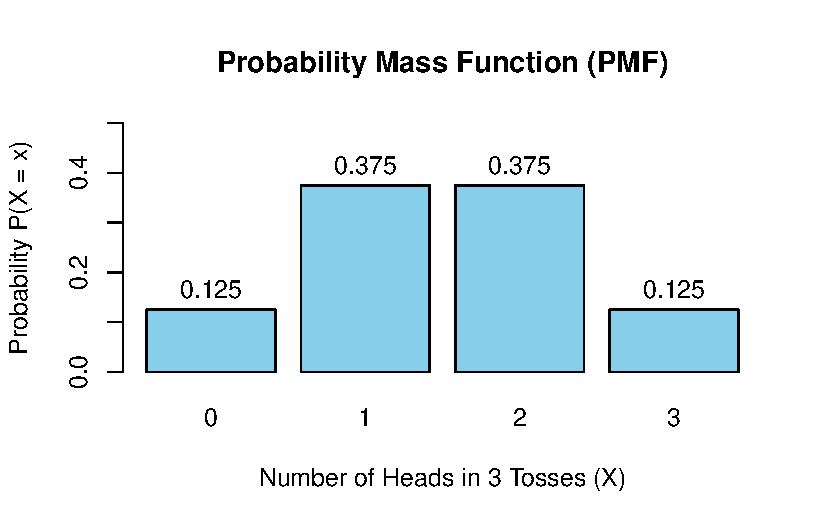
\includegraphics[keepaspectratio]{Ch8_files/figure-pdf/unnamed-chunk-1-1.pdf}}

The corresponding \textbf{cumulative probability distribution} can be
drawn as:

\pandocbounded{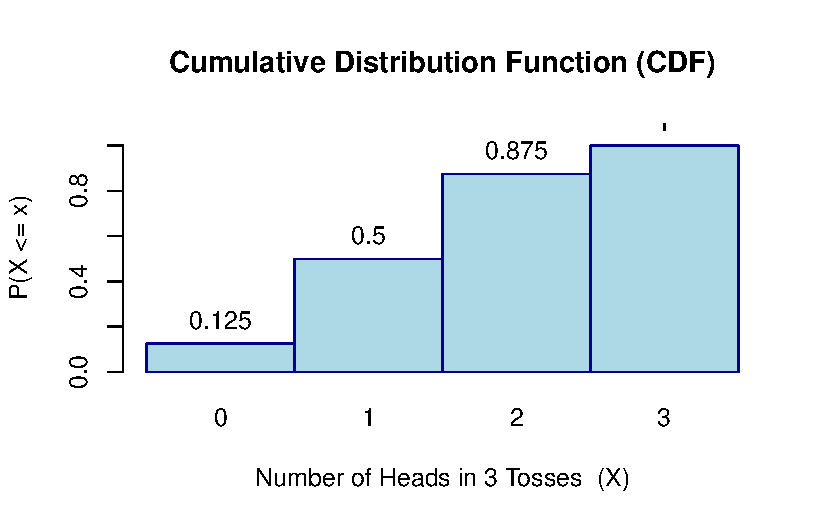
\includegraphics[keepaspectratio]{Ch8_files/figure-pdf/unnamed-chunk-4-1.pdf}}

\section{The mean and the variance}\label{the-mean-and-the-variance}

Apart from drawing the probability distribution or histograms, we have
seen that numerical summaries such as the mean and variance are useful.

The mean is the long-run average value of a random variable, which is
also referred to as its expected value, denoted \(E(X)\).

\begin{equation}\phantomsection\label{eq-expected-value}{
E(X) = \mu = \sum_{i=1}^{n} X_i P(X_i)
}\end{equation}

The variance which measures the spread or variation of the distribution
is defined as:

\begin{equation}\phantomsection\label{eq-variance}{
Var(X) = \sigma^2 = \sum_{i=1}^{n} (X_i- {\overline X})^2 P(X_i)
}\end{equation}

To get the standard deviation, simply calculate the square root of the
variance.

Let's see this with the example above which defines the random variable
\(X\) as the number of heads in 3 tosses.

To compute the mean, use Equation~\ref{eq-expected-value}, shown in the
table below--summing the last column of the table gives \(\mu = 1.5\).

\begin{table}

\caption{\label{tbl-mean}Calculating the mean.}

\centering{

\[
\begin{array}{|c|c|c|}
\hline
X & P(X) & X \cdot P(X) \\
\hline
0 & 1/8 & 0 \\
1 & 3/8 & 3/8 \\
2 & 3/8 & 6/8 \\
3 & 1/8 & 3/8 \\
\hline
\textbf{Total} & \mathbf{1} & \mathbf{12/8 = 1.5} \\
\hline
\end{array}
\]

}

\end{table}%

To get the variance, applying Equation~\ref{eq-variance}, as shown in
the the table below and summing the last column of the table gives
\(\sigma^2 = 0.75\)

\begin{table}

\caption{\label{tbl-variance}Calculating the variance.}

\centering{

\[
\begin{array}{|c|c|c|c|}
\hline
X & P(X) & (X_i - \mu) & (X_i - \mu)^2 \cdot P(X) \\
\hline
0 & 0.125 & -1.5 & 0.28125 \\
1 & 0.375 & -0.5 & 0.09375 \\
2 & 0.375 & 0.5 & 0.09375 \\
3 & 0.125 & 1.5 & 0.28125 \\
\hline
\mathbf{\Sigma} & \mathbf{1.000} & & \sigma^2 = \mathbf{0.75} \\
\hline
\end{array}
\]

}

\end{table}%

Careful, we have the variance \(=0.75\), hence the standard deviation
\(\sigma = \sqrt{0.75}\) which is about \(0.8667\).

\section{Rules of expected value and
variance}\label{rules-of-expected-value-and-variance}

Let us introduce some basic rules of expected value and variance.
Firstly, for \textbf{expected value}, we have:

\textbf{Rule E1} \[E(k)=k\] \textbf{Rule E2} \[E(X+k)=E(X)+k\]

\textbf{Rule E3} \[E(kX)=kE(X)\]

Rule \textbf{E1} states that the expected value (or average) of a
constant is that constant. Rule \textbf{E2} states that the expected
value of a random variable to which a constant has been added is equal
to the expected value of the random variable plus the constant. Rule
\textbf{E3} states that the expected value of a random variable
multiplied by a constant is equal to the constant times the expected
value of the random variable.

Secondly, the \textbf{rules of variance} are:

\textbf{Rule V1} \[Var(k)=0\]

\textbf{Rule V2} \[Var(X+k)=Var(X)\]

\textbf{Rule V3} \[Var(kX)=k^2 Var(X)\]

Rule \textbf{V1} states that the variance of a constant is zero (i.e.,
there is no spread). Rule \textbf{V2} states that the variance of a
random variable to which a constant has been added is simply equal to
the variance of the random variable. Lastly, Rule \textbf{V3} states
that the variance of a random variable multiplied by a constant is equal
to the constant squared times the variance of the random
variable.\^{}{[}It is instructive to compare the expected value and
variance rules with the summation rules.\footnote{It is instructive to
  compare the expected value and variance rules with the
  \textbf{summation} rules.}

\begin{tcolorbox}[enhanced jigsaw, coltitle=black, colbacktitle=quarto-callout-note-color!10!white, left=2mm, bottomrule=.15mm, bottomtitle=1mm, colback=white, titlerule=0mm, colframe=quarto-callout-note-color-frame, breakable, leftrule=.75mm, toptitle=1mm, opacitybacktitle=0.6, rightrule=.15mm, title=\textcolor{quarto-callout-note-color}{\faInfo}\hspace{0.5em}{Example: Monthly Profit Analysis}, arc=.35mm, opacityback=0, toprule=.15mm]

Let's illustrate how these rules apply to a real-world scenario.

\textbf{The Data:} For a food store, monthly sales have a mean (\(\mu\))
of \textbf{Baht 25,000} and a standard deviation (\(\sigma\)) of
\textbf{Baht 4,000}. Profits are defined as 30\% of sales minus fixed
costs of \textbf{Baht 6,000}.

\textbf{The Goal:} Find the mean and standard deviation of the monthly
profit.

\textbf{1. Define the Equation:} \[Profit = 0.30(Sales) - 6,000\]

\textbf{2. Calculate the Expected Value (Mean):}

\[
\begin{aligned}
V(\text{Profit}) &= V[0.30(\text{Sales}) - 6,000] \\
                 &= V[0.30(\text{Sales})]           && \text{(Rules V2 \& V1)} \\
                 &= (0.30)^2 V(\text{Sales})        && \text{(Rule V3)} \\
                 &= 0.09 \cdot (4,000)^2            \\
                 &= 0.09 \cdot 16,000,000           \\
                 &= 1,440,000
\end{aligned}
\]

\textbf{3. Calculate the Variance and Standard Deviation:} First, we
find the variance (\(V\)). Remember that
\(V(Sales) = \sigma^2 = 4,000^2\). \[
\begin{aligned}
V(\text{Profit}) &= V[0.30(\text{Sales}) - 6,000] \\
                 &= V[0.30(\text{Sales})]           && \text{(Rules V2 \& V1)} \\
                 &= (0.30)^2 V(\text{Sales})        && \text{(Rule V3)} \\
                 &= 0.09 \cdot (4,000)^2            \\
                 &= 0.09 \cdot 16,000,000           \\
                 &= 1,440,000
\end{aligned}
\]

Finally, the standard deviation is:
\[\sigma_{\text{Profit}} = \sqrt{1,440,000} = \mathbf{1,200}\]

\end{tcolorbox}

\section{Discrete bivariate
distributions}\label{discrete-bivariate-distributions}

So far, we have focused on \textbf{univariate distributions}. We now
extend these ideas to \textbf{bivariate probability distributions},
which arise from \textbf{joint probabilities}.

A \textbf{joint probability distribution} of two discrete random
variables \(X\) and \(Y\) is a table or formula that lists the joint
probabilities for all pairs of values \((x, y)\). It is denoted by
\(P(X,Y)\) or, equivalently, \(P(X = x \text{ and } Y = y)\).

As we would expect, joint probabilities satisfy the following basic
properties:

\(0 \le P(X,Y) \le 1\)

and

\(\sum_x \sum_y P(X,Y) = 1\).

\subsection{Joint and marginal
probabilities}\label{joint-and-marginal-probabilities}

We have already encountered an example of a bivariate probability
distribution in the previous chapter. That example involved a survey of
university graduates working as CEOs and whether they were \textbf{GA
graduates}.

The corresponding \textbf{joint} and \textbf{marginal} distributions are
summarized in the table below.

\begin{longtable}[]{@{}
  >{\raggedright\arraybackslash}p{(\linewidth - 6\tabcolsep) * \real{0.3088}}
  >{\raggedright\arraybackslash}p{(\linewidth - 6\tabcolsep) * \real{0.2059}}
  >{\raggedright\arraybackslash}p{(\linewidth - 6\tabcolsep) * \real{0.3235}}
  >{\raggedright\arraybackslash}p{(\linewidth - 6\tabcolsep) * \real{0.1618}}@{}}
\toprule\noalign{}
\begin{minipage}[b]{\linewidth}\raggedright
\end{minipage} & \begin{minipage}[b]{\linewidth}\raggedright
Becomes CEO
\end{minipage} & \begin{minipage}[b]{\linewidth}\raggedright
Does not becomes CEO
\end{minipage} & \begin{minipage}[b]{\linewidth}\raggedright
\textbf{Total}
\end{minipage} \\
\midrule\noalign{}
\endhead
\bottomrule\noalign{}
\endlastfoot
\textbf{GA graduate} & \(P(A_1 B_1)=0.11\) & \(P(A_1 B_2)=0.29\) &
\(P(A_1)=0.40\) \\
\textbf{Not GA graduate} & \(P(A_2 B_1)=0.06\) & \(P(A_2 B_2)=0.54\) &
\(P(A_2)=0.60\) \\
\textbf{Total} & \(P(B_1)=0.17\) & \(P(B_2)=0.83\) & \(1.00\) \\
\end{longtable}

\(A_1\) is the event that the individual is a GA graduate, or \(A_2\)
otherwise.\\
\(B_1\) is the event that the individual becomes a CEO, or \(B_2\)
otherwise.

The \textbf{marginal probabilities} are obtained by summing the joint
probabilities across rows or down columns. They describe the
probabilities of \(A\) and \(B\) \textbf{individually}, ignoring the
other variable.

Using marginal probabilities, we can compute the \textbf{mean},
\textbf{variance}, and \textbf{standard deviation} of each variable in a
bivariate distribution.

\subsubsection{\texorpdfstring{Marginal distribution of
\(A\)}{Marginal distribution of A}}\label{marginal-distribution-of-a}

\begin{table}

\caption{\label{tbl-marginal-A}Marginal Distribution of Event A}

\centering{

\[
\begin{array}{|c|c|}
\hline
A & P(A) \\
\hline
1 & 0.40 \\
0 & 0.60 \\
\hline
\end{array}
\]

}

\end{table}%

Using the expectation Equation~\ref{eq-expected-value} and variance
Equation~\ref{eq-variance} formulas introduced earlier:

\begin{itemize}
\tightlist
\item
  \(E(A) = 0.40\)
\item
  \(Var(A) = 0.24\)
\item
  \(SD(A) \approx 0.49\)
\end{itemize}

\subsubsection{\texorpdfstring{Marginal distribution of
\(B\)}{Marginal distribution of B}}\label{marginal-distribution-of-b}

Similarly, let \(B\) be an indicator variable that equals 1 if an
individual becomes a CEO and 0 otherwise. The marginal distribution of
\(B\) is:

\begin{table}

\caption{\label{tbl-marginal-B}Marginal Distribution of B}

\centering{

\[
\begin{array}{|c|c|}
\hline
B & P(B) \\
\hline
1 & 0.17 \\
0 & 0.83 \\
\hline
\end{array}
\]

}

\end{table}%

The corresponding \textbf{moments} are:\footnote{We will introduce the
  concept of moments later. Essentially the mean and variance are the
  first moments and second central moments, respectively.

  \[
  \begin{array}{|c|c|c|c|}
  \hline
  \text{Order} & \text{Raw Moment} & \text{Central Moment} & \text{Common Name} \\
  \hline
  \text{1st} & \mu_1' = E[X] & \mu_1 = E[X - E[X]] = 0 & \text{Mean} \\
  \hline
  \text{2nd} & \mu_2' = E[X^2] & \mu_2 = E[(X - \mu)^2] & \text{Variance} \\
  \hline
  \text{3rd} & \mu_3' & \mu_3 = E[(X - \mu)^3] & \text{Skewness} \\
  \hline
  \text{4th} & \mu_4' & \mu_4 = E[(X - \mu)^4] & \text{Kurtosis} \\
  \hline
  \end{array}
  \]}

\begin{itemize}
\tightlist
\item
  \(E(B) = 0.17\)
\item
  \(Var(B) \approx 0.14\)
\item
  \(SD(B) \approx 0.38\)
\end{itemize}

\subsection{Covariance of two discrete
variables}\label{covariance-of-two-discrete-variables}

We have already seen that the \textbf{covariance} between two discrete
random variables \(A\) and \(B\) is defined as

\begin{equation}\phantomsection\label{eq-covariance}{
Cov(A,B) = \sum_A \sum_B (A - \overline{A})(B - \overline{B}) P(A,B)
}\end{equation}

Continuing with the GA--CEO example, the covariance by
Equation~\ref{eq-covariance} between \(A\) and \(B\) is approximately

\(Cov(A,B) = 0.042\).

\subsection{Correlation}\label{correlation-1}

The \textbf{correlation coefficient} is obtained by dividing the
covariance by the product of the standard deviations:

\[
\text{Corr}(A,B) = \dfrac{\text{Covariance}(A,B)}{SD_A \, SD_B}
\] For this example, the correlation coefficient \(r \approx 0.23\).

We therefore conclude that there is a \emph{weak} \textbf{positive
relationship} between a GA graduate and becoming a CEO.

\section{The Binomial formula}\label{the-binomial-formula}

We have seen the multiplication and addition rules of probability.
Roughly speaking, these rules help us solve ``and'' and ``or'' problems.
Sometimes, however, we might wish to solve ``exact'' problems, for
example:

\begin{enumerate}
\def\labelenumi{\arabic{enumi}.}
\tightlist
\item
  A coin is tossed 4 times. What is the chance of getting exactly one
  head?
\item
  A die is rolled 10 times. What is the chance of getting exactly 3
  Aces?
\item
  A box contains one red marble and nine green ones. Five draws are made
  at random with replacement. What is the chance that exactly two draws
  will be red?
\end{enumerate}

It is with such problems that the binomial formula can be very helpful.

\subsection{Box Model Example}\label{box-model-example}

Let's look more closely at the last example above. We might start with a
box model:

\begin{figure}

\centering{

\pandocbounded{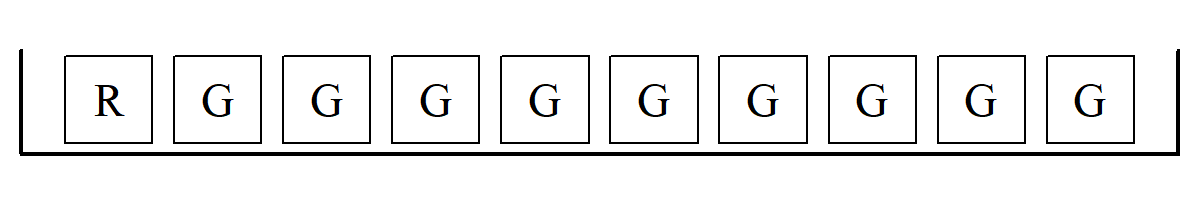
\includegraphics[keepaspectratio]{figs/ch8/r-g.png}}

}

\caption{\label{fig-r-g}Box Model}

\end{figure}%

From the above, we draw 5 tickets at random with replacement. But we
want exactly 2 R's and 3 G's (e.g.,
\(\fbox{R}, \fbox{R}, \fbox{G}, \fbox{G}, \fbox{G}\) or
\(\fbox{G}, \fbox{R}, \fbox{G}, \fbox{G}, \fbox{R}\), etc.). The exact
probability can be found using 3 simple steps:

\textbf{1) Find all the possible ways:} \[
\frac{5!}{2! \times 3!} = \frac{\text{total cases}}{\text{no. of successes} \times \text{no. of failures}}
\]

\textbf{2) Calculate the chance of each:} \[
\frac{1}{10} \times \frac{1}{10} \times \frac{9}{10} \times \frac{9}{10} \times \frac{9}{10} = \left( \frac{1}{10}\right)^2 \left( \frac{9}{10}\right)^3
\]

\textbf{3) Use the addition rule to add up the chances:} \[
\frac{5!}{2! \times 3!} \times \left( \frac{1}{10}\right)^2 \left( \frac{9}{10}\right)^3 \approx 7\%
\]

This can be interpreted as the chance of getting exactly 2
\(\fbox{R}\)'s.

Note that \textbf{step 1} is actually the \emph{binomial coefficient},
which gives us the total number of combinations of arranging 2 R's and 3
G's. In \textbf{step 2}, the chance of getting
\(\fbox{R}, \fbox{R}, \fbox{G}, \fbox{G}, \fbox{G}\) is the same as
getting \(\fbox{G}, \fbox{R}, \fbox{G}, \fbox{G}, \fbox{R}\), and so on.
Lastly, \textbf{step 3} involves the addition rules as all events are
mutually exclusive (disjoint).

\subsection{The Binomial Formula}\label{the-binomial-formula-1}

\begin{tcolorbox}[enhanced jigsaw, coltitle=black, colbacktitle=quarto-callout-important-color!10!white, left=2mm, bottomrule=.15mm, bottomtitle=1mm, colback=white, titlerule=0mm, colframe=quarto-callout-important-color-frame, breakable, leftrule=.75mm, toptitle=1mm, opacitybacktitle=0.6, rightrule=.15mm, title=\textcolor{quarto-callout-important-color}{\faExclamation}\hspace{0.5em}{The Binomial Formula}, arc=.35mm, opacityback=0, toprule=.15mm]

The chance that an event will occur exactly \(k\) times out of \(n\)
trials is given by

\begin{equation}\phantomsection\label{eq-binomial}{
P(X=k) = \frac{n!}{k!(n-k)!}p^k (1-p)^{n-k}, \text{ for } k = 0,1,\dots,n
}\end{equation}

Where: - \(n\) is the number of trials. - \(k\) is the number of times
the event of interest is to occur. - \(p\) is the probability that the
event of interest will occur on any particular trial.

\end{tcolorbox}

\textbf{Three conditions must hold for the binomial formula to be
valid:}

\begin{enumerate}
\def\labelenumi{\arabic{enumi}.}
\tightlist
\item
  The value of \(n\) must be fixed in advance.\\
\item
  \(p\) must be the same from trial to trial.\\
\item
  The trials must be independent of each other.
\end{enumerate}

\textbf{Quick Example}

To find the chance of getting exactly 2 aces in 10 rolls of a die:

\[
P(X=2) = \frac{10!}{2!8!}\left( \frac{1}{6} \right)^2 \left(\frac{5}{6} \right)^8 \approx 0.2907
\]

\section{The Poisson distribution}\label{the-poisson-distribution}

The Poisson random variable is a discrete random variable that typically
fits cases of rare events that occur over a fixed amount of time or
within a specified space or region. Typical cases are, for example:

\begin{itemize}
\tightlist
\item
  The number of customers entering a service station per hour.
\item
  The number of errors a typist makes per page.
\item
  The number of telephone calls received by a switchboard per hour.
\end{itemize}

\section{The Poisson Formula}\label{the-poisson-formula}

The Poisson probability distribution is given by:

\begin{equation}\phantomsection\label{eq-poisson}{
P(X=x) = f(x) = \frac{e^{-\mu} \mu^x}{x!}
}\end{equation}

Where: - \(\mu\) is the average number of successes in a particular
interval of time or space. - \(e\) is the constant
\(\approx 2.71828\dots\) - \(x\) is the number of successes.\^{}{[}Take
care of notation here. We have introduced \(f(x)\): the small ``\(f\)''
represents a probability density function.

Correspondingly, a large ``\(F\)'', say, \(F(x)\), would refer to the
cumulative probability function. This should be distinguished from the
large ``\(P\)'' we have been using, which stands for probability.{]}

\subsection{Assumptions of the Poisson
Process}\label{assumptions-of-the-poisson-process}

For the Poisson formula to be valid, the following conditions must be
met:

\begin{enumerate}
\def\labelenumi{\arabic{enumi}.}
\tightlist
\item
  \textbf{Independence}: The number of successes that occur in one time
  interval should be independent of the number of successes in another
  interval.
\item
  \textbf{Proportionality}: The probability of a success in a certain
  interval should be the same for all intervals of the same size and
  proportional to the length of the interval.
\item
  \textbf{Simultaneity}: The probability that two or more successes will
  occur in an interval approaches zero as the interval becomes smaller
  and smaller.
\end{enumerate}

\textbf{Example: Typographical Errors}

Assume that the number of typographical errors in a new edition of a
textbook follows a Poisson distribution with a mean of \textbf{1.5 per
100 pages}. If 100 pages are randomly selected, what is the probability
that there are no typos (\(X=0\))?

\[
\begin{aligned}
P(X=0) = f(0) &= \frac{e^{-1.5} 1.5^0}{0!} \\
              &= \frac{0.2231 \times 1}{1} \\
              &= \mathbf{0.2231}
\end{aligned}
\]

\section{Exercises}\label{exercises-4}

\subsection{Understanding discrete random
variables}\label{understanding-discrete-random-variables}

\begin{enumerate}
\def\labelenumi{\arabic{enumi}.}
\item
  \textbf{What is a discrete random variable?}\\
  Explain the difference between a \emph{random outcome} and a
  \emph{random variable}.\\
  Give two examples of discrete random variables drawn from everyday
  life.
\item
  \textbf{Probability distributions}\\
  A discrete random variable \(X\) takes values \(x_1, x_2, \dots, x_k\)
  with probabilities \(P(X=x_i)\).

  \begin{enumerate}
  \def\labelenumii{(\alph{enumii})}
  \tightlist
  \item
    What two conditions must a probability distribution satisfy?\\
  \item
    Explain in words why these conditions are necessary.
  \end{enumerate}
\end{enumerate}

\begin{center}\rule{0.5\linewidth}{0.5pt}\end{center}

\subsection{Mean, variance, and
transformations}\label{mean-variance-and-transformations}

\begin{enumerate}
\def\labelenumi{\arabic{enumi}.}
\setcounter{enumi}{2}
\item
  \textbf{A simple distribution}\\
  The random variable \(X\) has the following distribution:

  \begin{longtable}[]{@{}lllll@{}}
  \toprule\noalign{}
  \(X\) & 0 & 1 & 2 & 3 \\
  \midrule\noalign{}
  \endhead
  \bottomrule\noalign{}
  \endlastfoot
  \(P(X)\) & 0.4 & 0.3 & 0.2 & 0.1 \\
  \end{longtable}

  \begin{enumerate}
  \def\labelenumii{(\alph{enumii})}
  \tightlist
  \item
    Compute \(E[X]\), \(\text{Var}(X)\), and the standard deviation of
    \(X\).\\
  \item
    Interpret the mean of \(X\) in words.
  \end{enumerate}
\item
  \textbf{Linear transformations}\\
  Suppose \(Y = 3X + 2\).

  \begin{enumerate}
  \def\labelenumii{(\alph{enumii})}
  \tightlist
  \item
    Use the laws of expectation and variance to compute \(E[Y]\) and
    \(\text{Var}(Y)\).\\
  \item
    Find the standard deviation of \(Y\).\\
  \item
    Explain why adding a constant affects the mean but not the variance.
  \end{enumerate}
\end{enumerate}

\begin{center}\rule{0.5\linewidth}{0.5pt}\end{center}

\subsection{Joint distributions, independence, and
correlation}\label{joint-distributions-independence-and-correlation}

\begin{enumerate}
\def\labelenumi{\arabic{enumi}.}
\setcounter{enumi}{4}
\item
  \textbf{Joint distribution}\\
  The joint probability distribution of \(X\) and \(Y\) is given below:

  \begin{longtable}[]{@{}llll@{}}
  \toprule\noalign{}
  & \(Y=-1\) & \(Y=0\) & \(Y=1\) \\
  \midrule\noalign{}
  \endhead
  \bottomrule\noalign{}
  \endlastfoot
  \(X=0\) & 0.1 & 0.1 & 0.1 \\
  \(X=2\) & 0.1 & 0.2 & 0.1 \\
  \(X=4\) & 0.1 & 0.1 & 0.1 \\
  \end{longtable}

  \begin{enumerate}
  \def\labelenumii{(\alph{enumii})}
  \tightlist
  \item
    Compute the marginal distributions of \(X\) and \(Y\).\\
  \item
    Show that \(E[XY] = E[X]E[Y]\).\\
  \item
    Conclude that \(X\) and \(Y\) are uncorrelated.\\
  \item
    Show that \(X\) and \(Y\) are \textbf{not independent}.
  \end{enumerate}

  \emph{Why does zero correlation not imply independence?}
\item
  \textbf{Another joint distribution}\\
  The joint distribution of \(X\) and \(Y\) is given by:

  \begin{longtable}[]{@{}llll@{}}
  \toprule\noalign{}
  & \(X=0\) & \(X=1\) & \(X=2\) \\
  \midrule\noalign{}
  \endhead
  \bottomrule\noalign{}
  \endlastfoot
  \(Y=1\) & \(1/6\) & \(1/6\) & \(1/6\) \\
  \(Y=-1\) & 0 & \(1/2\) & 0 \\
  \end{longtable}

  \begin{enumerate}
  \def\labelenumii{(\alph{enumii})}
  \tightlist
  \item
    Compute \(E[X]\) and \(E[Y]\).\\
  \item
    Are \(X\) and \(Y\) independent? Justify your answer.\\
  \item
    Compute \(\text{Cov}(X,Y)\) and determine whether the variables are
    correlated.
  \end{enumerate}
\end{enumerate}

\begin{center}\rule{0.5\linewidth}{0.5pt}\end{center}

\subsection{Counting and discrete probability
models}\label{counting-and-discrete-probability-models}

\begin{enumerate}
\def\labelenumi{\arabic{enumi}.}
\setcounter{enumi}{6}
\item
  \textbf{Families and children}\\
  Assume that the probability of a boy equals the probability of a girl,
  and that births are independent.

  \begin{enumerate}
  \def\labelenumii{(\alph{enumii})}
  \tightlist
  \item
    In families with \textbf{four children}, what proportion have more
    girls than boys?\\
  \item
    List all relevant outcomes explicitly.
  \end{enumerate}
\item
  \textbf{Comparing family sizes}\\
  Couple A has \textbf{three children}.\\
  Couple B has \textbf{five children}.

  \begin{enumerate}
  \def\labelenumii{(\alph{enumii})}
  \tightlist
  \item
    For each couple, compute the probability that there are more girls
    than boys.\\
  \item
    Is the probability higher for couple A, couple B, or the same?\\
  \item
    Explain the intuition behind your result.
  \end{enumerate}
\end{enumerate}

\begin{center}\rule{0.5\linewidth}{0.5pt}\end{center}

\subsection{Discrete distributions in
practice}\label{discrete-distributions-in-practice}

\begin{enumerate}
\def\labelenumi{\arabic{enumi}.}
\setcounter{enumi}{8}
\item
  \textbf{Guessing on a multiple-choice exam}\\
  A student randomly guesses on a 100-question multiple-choice test.
  Each question has four possible answers.

  \begin{enumerate}
  \def\labelenumii{(\alph{enumii})}
  \tightlist
  \item
    What is the expected number of correct answers?\\
  \item
    What is the standard deviation?\\
  \item
    If a student scores 35 out of 100, would you attribute this more to
    luck or skill? Explain briefly.\\
  \item
    Which event has higher probability: scoring \textbf{exactly 55\%},
    or scoring \textbf{more than 55\%}?
  \end{enumerate}
\item
  \textbf{Arrivals at an urgent care center}\\
  The mean number of arrivals at an urgent care facility is 4 per hour.
\end{enumerate}

\begin{enumerate}
\def\labelenumi{(\alph{enumi})}
\tightlist
\item
  Assuming arrivals follow a Poisson process, what is the probability of
  exactly 2 arrivals in one hour?\\
\item
  Explain why the Poisson distribution is appropriate in this context.
\end{enumerate}

\begin{enumerate}
\def\labelenumi{\arabic{enumi}.}
\setcounter{enumi}{10}
\tightlist
\item
  \textbf{Website traffic}\\
  Hits to a personal website occur randomly and independently, with an
  average of 4 hits per week.
\end{enumerate}

\begin{enumerate}
\def\labelenumi{(\alph{enumi})}
\tightlist
\item
  What is the probability of receiving 10 or more hits in one week?\\
\item
  What is the probability of receiving 20 or more hits over two weeks?
\end{enumerate}

\begin{enumerate}
\def\labelenumi{\arabic{enumi}.}
\setcounter{enumi}{11}
\tightlist
\item
  \textbf{Manufacturing defects}\\
  Flaws in a carpet occur randomly at a rate of one per 300 square feet.
\end{enumerate}

\begin{enumerate}
\def\labelenumi{(\alph{enumi})}
\tightlist
\item
  What distribution is appropriate for modeling the number of flaws?\\
\item
  What is the probability that an \(8 \times 10\) foot carpet contains
  \textbf{no flaws}?
\end{enumerate}

\begin{center}\rule{0.5\linewidth}{0.5pt}\end{center}

\subsection{Conceptual wrap-up}\label{conceptual-wrap-up}

\begin{enumerate}
\def\labelenumi{\arabic{enumi}.}
\setcounter{enumi}{12}
\tightlist
\item
  \textbf{Big picture}
\end{enumerate}

\begin{enumerate}
\def\labelenumi{(\alph{enumi})}
\tightlist
\item
  How do discrete probability distributions help us model uncertainty?\\
\item
  Why are expectations and variances central to economic analysis?\\
\item
  Give one example from economics where a discrete random variable is
  more appropriate than a continuous one.
\end{enumerate}

\phantomsection\label{refs}
\begin{CSLReferences}{1}{0}
\bibitem[\citeproctext]{ref-efron1998fisher}
Efron, Bradley. 1998. {``R. A. Fisher in the 21st Century.''}
\emph{Statistical Science} 13 (2): 95--122.
\url{https://doi.org/10.1214/ss/1028905930}.

\end{CSLReferences}




\end{document}
